\documentclass[journal]{IEEEtran}
\IEEEoverridecommandlockouts

\usepackage[utf8]{inputenc}
\usepackage[T1]{fontenc}
\usepackage{amsmath,amssymb}
\usepackage{graphicx}
\usepackage{booktabs}
\usepackage{multirow}
\usepackage{url}
\usepackage{xcolor}
\usepackage{microtype}
\usepackage{cite}
\usepackage{array}
\usepackage[caption=false,font=footnotesize]{subfig}
\usepackage{pdflscape}
\usepackage{rotating}
\usepackage{threeparttable}

% Highlight best results
\newcommand{\best}[1]{\textbf{#1}}
\newcommand{\snd}[1]{\underline{#1}}
\newcommand{\tbd}[1]{\textit{#1}\textsuperscript{\dag}}   % placeholder for pending (in-progress) results

\begin{document}

\title{Cross-Linguistic Isolated Sign Language Recognition with Skeletal Gait Energy Images and Multi-Scale Kinematic Descriptors: A Study on Libras, ASL, and BSL}

\author{
  Jonathan~N.~Gois,~Miqueas~dos~S.~Pinheiro,~Wesley~L.~Passos,~Gabriel~M.~Araujo,\\
  Felipe~da~R.~Henriques,~Alessandro~R.~L.~Zachi,~and~Amaro~A.~Lima
  \thanks{J. N. Gois and W. L. Passos are with CEFET/RJ, Campus Nova Iguaçu, and with PESC/COPPE, Universidade Federal do Rio de Janeiro (UFRJ), Rio de Janeiro, Brazil.}
  \thanks{M. dos S. Pinheiro, W. L. Passos, G. M. Araujo, and A. R. L. Zachi are with PPEEL/CEFET-RJ, Rio de Janeiro, Brazil.}
  \thanks{F. da R. Henriques is with CEFET/RJ, Campus Petrópolis, and with PPGIO/PPCIC-CEFET/RJ, Rio de Janeiro, Brazil.}
  \thanks{A. A. Lima is with CEFET/RJ and PPGIO/CEFET-RJ, Rio de Janeiro, Brazil.}
  \thanks{Manuscript draft, \today. This manuscript extends a conference paper accepted at SBrT 2026 (Classificação de Sinais Isolados em Libras com Descritores Cinemáticos e Gait Energy Image), restricted to Libras/MINDS-Libras, with (i) a cross-linguistic evaluation on American Sign Language (ASL) and British Sign Language (BSL), (ii) a leave-one-signer-out (LOPO) protocol used uniformly across all three languages, and (iii) an extensive ablation study not present in the conference version. Entries marked \tbd{pending} indicate results for which the data-acquisition and training pipeline is fully specified but not yet complete -- as of this draft, limited to leave-one-signer/source-out evaluation of the five deep-sequence models on ASL/BSL (deferred as future work, Section~\ref{sec:limitations}) and the cross-linguistic Wilcoxon significance tests; see Section~\ref{sec:limitations} for a full disclosure of what is and is not final in this draft.}
}

\markboth{Draft for IEEE Access}{Gois \MakeLowercase{\textit{et al.}}: Cross-Linguistic Isolated Sign Language Recognition}

\maketitle

% ─────────────────────────────────────────────────────────────────────────────
\begin{abstract}
Isolated sign language recognition (ISLR) systems are usually developed and validated on a single language and a single dataset, which makes it difficult to know whether a proposed representation captures properties of manual communication in general or artifacts of one corpus. This paper extends a skeleton-based methodology combining a proposed \emph{skeletal Gait Energy Image} (GEI), multi-scale kinematic descriptors (position, velocity, acceleration, and spectral components), and Kalman-filtered landmark trajectories, originally validated on Brazilian Sign Language (Libras) using the MINDS-Libras dataset, to two additional, independently collected, widely used sign language corpora: WLASL (American Sign Language, ASL) and BSLDict (British Sign Language, BSL). Libras and ASL are evaluated under a common leave-one-signer-out (LOPO) protocol; BSL is evaluated under a leave-one-source-out (LOSO) protocol using the closest available grouping field in its metadata, since direct inspection confirmed BSLDict does not ship a true per-clip signer identifier (Section~\ref{sec:datasets}) -- this distinction is disclosed explicitly rather than treating LOSO as equivalent to LOPO. All three protocols are applied in addition to the two within-signer protocols used in prior Libras work (stratified hold-out and stratified $10$-fold cross-validation), so that generalization to unseen signers -- not merely to unseen samples -- can be measured and compared across languages. On MINDS-Libras, the corrected and extended pipeline reaches up to $98.91\%\pm0.76\%$ accuracy under within-signer 10-fold validation and $75.90\%\pm16.44\%$ under LOPO with 12 signers, matching or exceeding two literature baselines (Passos~et~al., GEI+SVM, $84.66\%$; Rego~et~al., FFT+kinematics+BiLSTM, $92.0\%$/$77.01\%$ LOPO with 8 signers). We additionally report an extensive ablation across feature modalities (GEI-only, kinematics-only, spectral-only, and their combinations), four classical classifiers (SVM, MLP, Extra Trees, Random Forest), five deep sequence models, two temporal-smoothing strategies (Kalman filtering versus exponential moving average), and a data-augmentation study that identifies mirror augmentation as \emph{harmful} for Libras due to phonological handedness -- more configurations than are needed for a final camera-ready table, so that the strongest, most defensible subset can be selected during revision. Results on ASL (WLASL) and BSL (BSLDict), collected and processed with the identical streaming acquisition-extraction pipeline and landmark normalization used for Libras, are reported where available at submission time and otherwise marked as pending, with the complete experimental protocol specified so that the cross-linguistic comparison can be finalized without re-deriving methodology.
\end{abstract}

\begin{IEEEkeywords}
Sign language recognition, isolated sign classification, Libras, American Sign Language, British Sign Language, gait energy image, kinematic descriptors, Kalman filter, leave-one-signer-out, cross-linguistic generalization.
\end{IEEEkeywords}

% ═════════════════════════════════════════════════════════════════════════════
\section{Introduction}
\label{sec:intro}

Sign languages are complete, natural languages with their own phonology, morphology, and syntax, used as a primary means of communication by Deaf and hard-of-hearing communities worldwide~\cite{quadros2004}. Brazilian Sign Language (Libras) is the legally recognized language of the Brazilian Deaf community~\cite{lei2002}, used by a population of several million people according to the last national census~\cite{ibge2010}; American Sign Language (ASL) and British Sign Language (BSL) play analogous roles in the United States/English-Canada and in the United Kingdom, respectively. Despite serving comparable communicative functions, these three languages are historically and structurally distinct -- BSL and ASL, in particular, are mutually unintelligible despite both being used in English-speaking countries, since ASL derives from French Sign Language while BSL belongs to the separate BANZSL family. Automatic sign language recognition (SLR) systems can support assistive technologies, educational tools, and communication mediation between signing and non-signing individuals~\cite{costa2025review,cheok2019review}, but the overwhelming majority of published ISLR systems are designed, tuned, and validated on a single dataset in a single language, leaving open the question of whether a given representation is discriminative because it captures general properties of manual articulation, or because it overfits idiosyncrasies of one corpus, one camera setup, or one group of signers.

Automatic sign recognition is challenging because sign languages combine manual components (handshape, orientation, spatial location, movement) with non-manual components (facial expression, mouthing, body posture)~\cite{cheok2019review}. Even for isolated signs, where each sample corresponds to a single lexical unit with well-defined onset and offset, classification is non-trivial: distinct signs may share handshape, trajectory, or place of articulation, while the same sign may vary in amplitude, speed, motor style, and body positioning across signers~\cite{rastgoo2021,sarhan2023islr}. Video-based methods are attractive because they are accessible and non-invasive, but they inherit visual noise, occlusion, illumination variation, and background/camera dependence~\cite{cheok2019review}. Deep architectures based on convolutional, recurrent, and attention mechanisms have achieved strong results on several sign benchmarks~\cite{rastgoo2021,sarhan2023islr,wadhawan2020static}, but typically require large annotated corpora, expensive training, and considerable computational capacity. For Libras specifically, the scarcity of large, standardized, diverse datasets is even more salient~\cite{costa2025review}, and the same holds, to varying degrees, for most sign languages other than ASL.

Given data scarcity and the complexity of the signal, compact representations of the signal to be classified are attractive from both a modeling and a computational-cost perspective. The \emph{Gait Energy Image} (GEI), originally proposed for gait-based person identification, compresses a temporal sequence of silhouettes into a single average image, preserving the spatial distribution of recurring motion~\cite{han2006gei}. In prior work, this concept was adapted to Libras recognition, exploring energy-based compact representations on datasets such as CEFET/RJ-Libras, MINDS-Libras, and LIBRAS-UFOP~\cite{passos2021}. While efficient, GEI tends to lose fine-grained temporal information, since frame aggregation attenuates differences in velocity, acceleration, and angular variation along the gesture. To address this limitation, kinematic statistics extracted from body and hand landmark trajectories were introduced, describing motion dynamics through position, velocity, acceleration, and spectral components~\cite{rego2025}. Because pose estimators can produce noise, jitter, and tracking failures, a Kalman filter is applied to landmark trajectories before feature extraction, reducing frame-to-frame instability without removing the dominant dynamics of the sign~\cite{kalman1960,wan2023kalman}.

The conference version of this work~[SBrT~2026, accepted] combined a \emph{skeletal} GEI -- rendered from normalized body and hand landmarks rather than from dense body-part masks or silhouettes -- with multi-scale kinematic descriptors and Kalman smoothing, and evaluated the combination on MINDS-Libras under two within-signer protocols, reaching accuracies up to $98.91\%$ and outperforming two Libras-specific literature baselines~\cite{passos2021,rego2025}. That evaluation, however, left two questions open. First, both validation protocols split by \emph{sample}, not by \emph{signer}: videos from the same signer can appear in both training and test partitions across different splits, so the reported accuracies primarily measure within-signer discrimination rather than generalization to unseen signers -- a limitation explicitly acknowledged in the conference paper as future work. Second, the methodology was validated on a single language; whether the same skeletal-GEI-plus-kinematics representation is discriminative for signs beyond Libras' particular phonological inventory (e.g., its comparatively frequent two-handed, symmetric signs) was left unanswered.

This paper addresses both points. We adopt a signer-independent, leave-one-signer-out (LOPO) protocol as the primary evaluation criterion across all experiments, in addition to reporting the two within-signer protocols used previously for direct comparability with prior Libras literature. We then apply the identical extraction, normalization, Kalman-smoothing, skeletal-GEI, and kinematic-descriptor pipeline -- without language-specific tuning -- to two additional isolated-sign corpora: WLASL, the most widely used large-vocabulary ASL benchmark~\cite{wlasl2020}, and BSLDict, a British Sign Language dictionary corpus with multiple signers per sign, released by the University of Oxford's Visual Geometry Group under a CC-BY~4.0 license~\cite{momeni2020bsldict}. The choice of BSLDict over the larger, more frequently cited BOBSL/BSL-1K corpora~\cite{albanie2020bsl1k,albanie2021bobsl} is a deliberate, disclosed methodological decision, discussed in Section~\ref{sec:datasets}: BOBSL requires a bilateral data-sharing agreement with the BBC with an unbounded approval timeline, and even its pose-only release ($\approx$591~GiB) is two orders of magnitude larger than what is required by an isolated-sign, skeleton-only pipeline such as ours, whereas BSLDict is immediately and legally downloadable, is sourced from the same research group, and -- like MINDS-Libras and WLASL -- is structured as isolated signs performed by multiple signers, which is the setting our methodology targets.

In summary, the contributions of this work are:
\begin{itemize}
\item A skeletal adaptation of the Gait Energy Image built from normalized body and hand landmarks (rather than from body-part masks or silhouettes), evaluated, for the first time in this line of work, under a signer-independent protocol.
\item Multi-scale kinematic descriptors -- position, velocity (at three temporal scales), acceleration, and spectral magnitude/phase -- extracted from Kalman-filtered landmark trajectories, and a systematic ablation isolating the contribution of each descriptor family.
\item A LOPO protocol applied uniformly to three independent, structurally comparable isolated-sign corpora in three different sign languages (Libras/MINDS-Libras, ASL/WLASL, BSL/BSLDict), enabling, for the first time in this line of work, a same-methodology comparison of signer-independent generalization across languages.
\item A streaming acquisition pipeline (download $\rightarrow$ MediaPipe landmark extraction $\rightarrow$ discard raw video) reused from an existing large-scale Libras data-collection effort~\cite{lugaresi2019mediapipe} and adapted to WLASL and BSLDict, chosen specifically to make the multi-corpus, multi-language extension feasible under tight local-storage constraints without ever requiring the raw video corpus to be held on disk.
\item An extensive experimental study -- eleven classifier/feature configurations, five deep sequence models, an augmentation study, a temporal-smoothing study, and a dimensionality-reduction study, all on Libras, with the identical protocol grid specified for ASL and BSL -- deliberately larger than what a camera-ready IEEE Access paper is expected to retain, so that the strongest and most defensible subset of results can be selected during revision (Section~\ref{sec:limitations}).
\end{itemize}

The remainder of this paper is organized as follows. Section~\ref{sec:related} reviews related work in ISLR, GEI-based recognition, kinematic/spectral descriptors, and the ASL/BSL dataset landscape. Section~\ref{sec:methodology} describes the proposed methodology. Section~\ref{sec:datasets} describes the three datasets and the acquisition pipeline used for ASL and BSL. Section~\ref{sec:setup} describes the experimental protocols and classifiers. Section~\ref{sec:results} reports results, organized as a set of independent experiments so that unwanted configurations can be pruned without breaking the narrative. Section~\ref{sec:discussion} discusses cross-linguistic findings. Section~\ref{sec:limitations} discloses, explicitly, the current status of every result in the paper. Section~\ref{sec:conclusion} concludes.

% ═════════════════════════════════════════════════════════════════════════════
\section{Related Work}
\label{sec:related}

\subsection{Isolated and continuous sign language recognition}
SLR is commonly divided into isolated sign language recognition (ISLR), where each sample corresponds to a single lexical unit with known boundaries, and continuous sign language recognition (CSLR), where a video must be mapped to a sequence of glosses, typically via connectionist temporal classification (CTC)~\cite{koller2020survey,phoenix2014}. Even though isolated recognition is, in principle, an easier problem, it remains far from solved for languages with limited annotated data, and it is a necessary building block for CSLR pipelines that rely on sign spotting or gloss dictionaries~\cite{momeni2020bsldict}. Recent CSLR literature has moved toward lightweight temporal mixing to replace expensive 3D convolutions~\cite{jiang2026}, learned Kalman-fusion gates for robustness to landmark noise~\cite{zhang2024}, and sparse, keyframe-anchored graph attention to reduce temporal redundancy~\cite{ye2026}. These three directions -- lightweight mixing, filtering, and sparse/salient temporal modeling -- motivate, respectively, our use of compact per-frame descriptors, our use of Kalman smoothing prior to feature extraction, and our saliency-weighted GEI variant (Section~\ref{sec:methodology}).

\subsection{GEI-based and skeleton-based representations}
The Gait Energy Image was originally proposed for gait-based person re-identification, compressing a silhouette sequence into a single average image~\cite{han2006gei}. Its adaptation to sign recognition compresses the spatial envelope of hand and body motion into a compact 2D descriptor, and was previously evaluated on Libras using dense body-part masks~\cite{passos2021}, achieving $84.66\%$ on a stratified hold-out protocol on MINDS-Libras. Skeleton-based representations more broadly -- as opposed to RGB- or mask-based ones -- have become dominant in recent SLR literature because they are robust to background and appearance variation and are compatible with lightweight, real-time pose estimators such as MediaPipe Holistic~\cite{lugaresi2019mediapipe,goyal2023mediapipe,lin2023mediapipe}. The present work follows this trend, replacing the dense-mask GEI of~\cite{passos2021} with a GEI rendered directly from normalized MediaPipe landmarks, which we refer to as \emph{skeletal GEI}.

\subsection{Kinematic and spectral descriptors}
An alternative to spatial-envelope compression is to describe motion dynamics directly through position, velocity, acceleration, and frequency-domain statistics of landmark trajectories. This direction was explored for Libras with a fast Fourier transform (FFT)-based kinematic pipeline feeding a BiLSTM classifier, reaching $92.0\%\pm3.00\%$ accuracy under $10$-fold cross-validation and $77.01\%\pm$ (unspecified std.) under a leave-some-signers-out protocol restricted to $8$ of the dataset's signers~\cite{rego2025}. Our kinematic branch follows the same family of descriptors (multi-scale velocity, acceleration, spectral magnitude and phase) but is evaluated with classical supervised classifiers rather than a recurrent network, and under LOPO with all available signers rather than a subset.

\subsection{Kalman filtering for pose-based recognition}
Kalman filtering has been used to smooth noisy skeleton trajectories in human action recognition~\cite{wan2023kalman} and, more recently, as a learned fusion gate inside CSLR pipelines~\cite{zhang2024}. Our filter is the classical scalar random-walk Kalman filter~\cite{kalman1960}, applied independently to each of the $225$ landmark coordinates in a single causal pass, without a learned gate; we retain the name ``Kalman filter'' rather than ``DKF'' throughout this paper to avoid the naming collision with the gated Dynamic Kalman Fusion of~\cite{zhang2024} present in the codebase's earlier internal reports.

\subsection{Libras-specific literature and datasets}
MINDS-Libras~\cite{rezende2021minds} is a controlled-recording dataset of $1\,560$ samples across $20$ lexical classes and $12$ signers, five repetitions per sign. It has been used as a benchmark by a $3$D-CNN system combining RGB, depth, and skeleton streams ($93.3\%$), a RGB-only 3D CNN ($96.0\%$)~\cite{decastro2022}, a FastDTW-based classifier ($\approx96\%$), and the two direct baselines already discussed~\cite{passos2021,rego2025} -- but none of these four report a signer-independent (LOPO) protocol, so they are only comparable to our within-signer Protocol-A/B numbers (Table~\ref{tab:core_protab}), not to our primary LOPO metric. Critically, three more recent works \emph{do} report LOPO/nested-LOPO on the identical MINDS-Libras 12-signer, 20-class configuration we use, and set a substantially higher bar than~\cite{rego2025}'s $77.01\%$ (8 signers): De Castro et al.~\cite{decastro2023skeleton} reach $91\%\pm7\%$; Alves et al.~\cite{alves2024skeleton} reach $93\%\pm5\%$ accuracy/F1 using a skeleton-sequence-as-2D-image representation fed to an ImageNet-pretrained CNN (rather than collapsing the sequence into a single GEI or globally aggregated kinematic statistics, as this paper's classical pipeline does); and dos Santos et al.~\cite{dossantos2025landmarksubset} refine the same representation with a landmark-subset-selection step to reach $F1=0.94$. Our own best LOPO result ($75.90\%\pm16.44\%$, Table~\ref{tab:lopo_libras}) is therefore \emph{below}, not above, the current published state of the art under this protocol; Section~\ref{ssec:skeleton_cnn} reports our attempt to close this gap by adapting the same skeleton-image-plus-CNN idea to our pipeline, and Section~\ref{sec:limitations} discloses this comparison explicitly rather than omitting it. A cross-dataset study on Brazilian Sign Language translation found that MediaPipe-landmark-plus-LSTM pipelines generalize substantially better across Libras corpora than CNNs applied directly to RGB ($75.5\%$ vs.\ $41\%$ top-5)~\cite{sarmento2023}, which further motivates the landmark-based approach adopted here. A recent systematic review of AI-based Libras recognition highlights the scarcity of large, standardized, cross-signer-evaluated Libras datasets as an open problem in the field~\cite{costa2025review}, which this paper's LOPO protocol directly targets.

\subsection{ASL datasets}
American Sign Language is the best-resourced sign language for computer-vision research. WLASL~\cite{wlasl2020} is, at the time of writing, the most widely used large-vocabulary ISLR benchmark for ASL, comprising $21\,083$ video instances across $2\,000$ gloss classes performed by more than $100$ signers, sourced from YouTube and educational ASL dictionaries, and released with explicit per-instance signer identifiers that directly support signer-independent evaluation. MS-ASL~\cite{joze2019msasl} is a comparable large-scale alternative ($1\,000$ classes, $200$+ signers) and is cited here to contextualize the scale of ASL resources relative to Libras and BSL, but was not selected as the primary ASL corpus because WLASL has, by a wide margin, the larger footprint in the recent ISLR literature and provides pre-extracted body keypoints alongside raw video, which further reduces the acquisition burden. Beyond the RGB-based I3D baseline originally released with WLASL, the pose/skeleton-only track of the ASL ISLR literature -- Pose-GRU and Pose-TGCN~\cite{wlasl2020}, SPOTER~\cite{bohacek2022spoter,bohacek2022mediapipe}, the skeleton branch of SAM-SLR-v2~\cite{jiang2021samslr}, and, most recently, the dual-stream graph-convolutional DSLNet~\cite{liu2025dslnet} ($93.70\%$ WLASL100, $89.97\%$ WLASL300, skeleton-only, published 2025) -- is the more methodologically comparable body of work to the present study, since none of it consumes RGB appearance; Section~\ref{sec:asl_bsl_results} compares our WLASL results against all of these rather than against I3D alone. DSLNet's result is included specifically to keep this comparison current: it roughly doubles SPOTER's WLASL100 accuracy two to three years later, which is itself informative about how fast the skeleton-only WLASL state of the art has moved and is a caution against treating any single-year snapshot of ``the'' SOTA as stable.

\subsection{BSL datasets}
British Sign Language resources are comparatively scarce and structurally different from the ASL landscape. BSL-1K~\cite{albanie2020bsl1k} and its public extension BOBSL~\cite{albanie2021bobsl} are, respectively, the largest co-articulated and continuous BSL video corpora, sourced from BBC broadcast footage; both require a signed data-sharing agreement with the BBC, and BOBSL's full release, even restricted to pre-extracted pose estimations, is $\approx$591~GiB -- roughly two orders of magnitude larger than what an isolated-sign, skeleton-only ISLR pipeline requires, and infeasible to acquire under the storage budget available for this study (Section~\ref{sec:datasets}). BSLDict~\cite{momeni2020bsldict}, released by the same research group and sourced from the public BSL dictionary aggregator signbsl.com, is structured as isolated dictionary entries ($9\,283$ signs, $14\,210$ clips, $28$+ signers) rather than continuous broadcast footage, is distributed under a CC-BY~4.0 license without an approval process, and is therefore the BSL corpus used in this study. We are not aware of prior work evaluating a GEI-plus-kinematics pipeline on BSLDict, or of prior work directly comparing signer-independent ISLR accuracy across Libras, ASL, and BSL under a shared methodology; to our knowledge, this is the first study to do so.

% ═════════════════════════════════════════════════════════════════════════════
\section{Methodology}
\label{sec:methodology}

The methodology is organized into four stages, applied identically to all three languages: (i)~landmark extraction and normalization, (ii)~Kalman temporal smoothing, (iii)~skeletal-GEI construction, and (iv)~kinematic-feature extraction from the smoothed trajectories. No language-specific parameter was tuned; the only per-corpus adaptation is the acquisition front-end described in Section~\ref{sec:datasets}, since raw video for WLASL and BSLDict must be streamed and discarded rather than stored in bulk. Fig.~\ref{fig:pipeline} summarizes the four stages.

\begin{figure}[t]
\centering
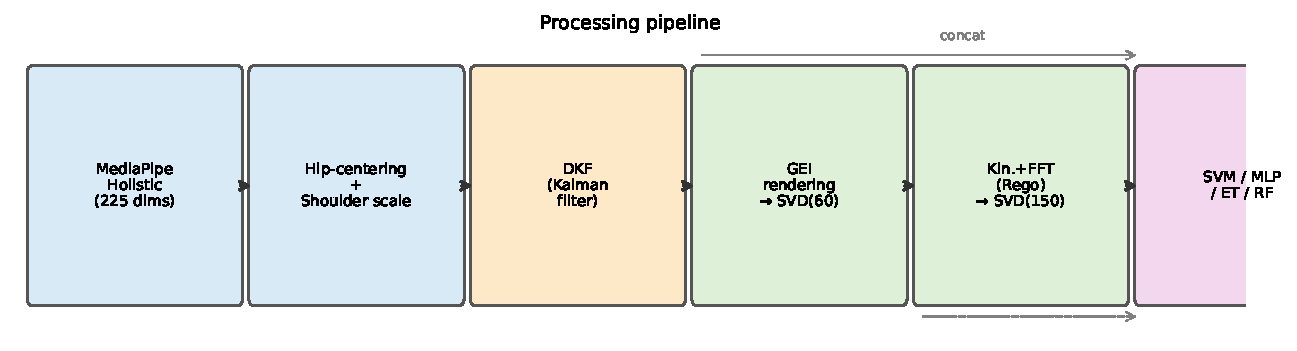
\includegraphics[width=\columnwidth]{results/fig_pipeline.pdf}
\caption{Overview of the proposed pipeline: landmark extraction and normalization, Kalman smoothing, skeletal-GEI rendering, and multi-scale kinematic feature extraction. Applied identically to Libras, ASL, and BSL.}
\label{fig:pipeline}
\end{figure}

\subsection{Landmark extraction and normalization}
For each input video, body and hand landmarks are extracted with MediaPipe Holistic~\cite{lugaresi2019mediapipe}. Each frame is initially represented as a matrix $\mathbf{S}_t \in \mathbb{R}^{75\times3}$, $t=1,\dots,T$, where $T$ is the number of frames. The $75$ points correspond to $33$ body-pose landmarks and $21$ landmarks for each hand, each described by coordinates $(x,y,z)$. The $x$ and $y$ coordinates correspond to normalized image-plane positions, while $z$ represents MediaPipe's relative depth estimate. After spatial centering in $x$ and $y$, the $z$ coordinate is scaled by the same body-derived factor used for the other coordinates so that all three components lie in comparable ranges. For Kalman smoothing, saliency computation, and kinematic-feature extraction, this matrix is vectorized as $\mathbf{s}_t \in \mathbb{R}^{225}$. Coordinates are normalized per sequence to mitigate global position and scale variation: in each frame, points are centered at the midpoint of the hips (landmarks 23 and 24), and the whole sequence is then scaled by the average shoulder-to-shoulder distance over the video, applied identically to $x$, $y$, and $z$.

\subsection{Kalman filtering}
Pose-estimator trajectories can exhibit noise, jitter, and tracking failures, particularly under occlusion, fast motion, low resolution, or lighting variation. These artifacts are especially damaging to kinematic features, since velocity and acceleration are computed by temporal differencing and tend to amplify frame-to-frame variation. Each of the $225$ normalized coordinates is filtered independently by a scalar random-walk Kalman model~\cite{kalman1960}. Letting $y_t$ be the observed coordinate at time $t$ and $x_t$ the corresponding smoothed state,
\begin{equation}
x_t = x_{t-1} + w_t, \qquad y_t = x_t + \nu_t,
\label{eq:kalman}
\end{equation}
with $w_t\sim\mathcal{N}(0,Q)$ and $\nu_t\sim\mathcal{N}(0,R)$. We adopt $Q=10^{-4}$ and $R=5\times10^{-3}$, producing moderate smoothing; prediction and update follow the standard scalar Kalman recursion. Filtering is performed in a single causal forward pass (no backward smoothing), and is initialized at the first frame with non-degenerate norm, $t_0=\min\{t:\|\mathbf{s}_t\|_2>10^{-6}\}$, to avoid biasing the filter with a null vector when early frames fail detection.

\subsection{Skeletal Gait Energy Image}
Each normalized, smoothed frame is converted into a binary skeleton image $\mathbf{F}_t\in\{0,1\}^{H\times W}$, $H=64$, $W=48$, by projecting body and hand landmarks onto the $(x,y)$ plane and drawing the anatomical connections between adjacent joints. A fixed spatial window $[p_{\min},p_{\max}]=[-4,4]$ is used after body normalization (rather than a per-frame rescaling), preserving relative amplitude and displacement differences across the sequence and avoiding artificial compression or expansion of signs with different spatial extents. Pixel coordinates for column and row are
\begin{align}
c_{t,j} &= \left\lfloor (W-1)\,\frac{\mathrm{clip}(p^x_{t,j},p_{\min},p_{\max})-p_{\min}}{p_{\max}-p_{\min}} \right\rfloor, \\
r_{t,j} &= \left\lfloor (H-1)\left(1-\frac{\mathrm{clip}(p^y_{t,j},p_{\min},p_{\max})-p_{\min}}{p_{\max}-p_{\min}}\right) \right\rfloor,
\label{eq:gei_pixel}
\end{align}
where $\mathrm{clip}(\cdot)$ bounds the value within the pre-established limits. The uniform GEI is the temporal average of rendered frames, $\mathbf{G}_{\mathrm{unif}}=\frac{1}{T}\sum_{t=1}^{T}\mathbf{F}_t$. Because this weights static and highly dynamic instants equally, we additionally compute a saliency-weighted variant. Defining the frame-to-frame displacement $d_t=\|\mathbf{s}_t-\mathbf{s}_{t-1}\|_2$ for $t=2,\dots,T$, weights are $\omega_t = d_t / (\sum_{\tau=2}^{T}d_\tau+\epsilon)$, with $\omega_1=\omega_2$ and $\epsilon>0$; the saliency-weighted GEI is $\mathbf{G}_{\mathrm{sal}} = \sum_{t=1}^{T}\omega_t\mathbf{F}_t / (\sum_{t=1}^{T}\omega_t+\epsilon)$. The resulting descriptor, vectorized, has dimension $H\times W = 3\,072$, and is used either alone or concatenated with the kinematic descriptor. Unlike~\cite{passos2021}, which computes the energy image from dense body-part masks, this work renders skeletons from normalized anatomical landmarks, preserving the relative geometry of motion rather than the appearance of the signer.

\subsection{Kinematic feature extraction}
Let $\mathbf{s}_t\in\mathbb{R}^{225}$ be the coordinate vector of the $75$ three-dimensional landmarks at time $t$, after normalization and smoothing. The position component is simply $\mathbf{p}_t=\mathbf{s}_t$. Velocities are computed by multi-scale differencing,
\begin{equation}
\mathbf{v}_t^{(\delta)} = \mathbf{s}_t - \mathbf{s}_{t-\delta}, \qquad \delta \in \{1,2,4\},
\label{eq:vel}
\end{equation}
capturing both fast, adjacent-frame displacement and coarser motion over longer intervals. Acceleration is a second-order difference, $\mathbf{a}_t = \mathbf{s}_{t+1} - 2\mathbf{s}_t + \mathbf{s}_{t-1}$, with edge replication at sequence boundaries. Spectral features are computed with a Hann-windowed FFT over a local temporal window of length $L_{\mathrm{fft}} = \min(\max(\lfloor T/\alpha\rfloor, L_{\min}), L_{\max})$, $\alpha=4$, $L_{\min}=16$, $L_{\max}=64$, with edge padding to keep window length constant across the sequence; for each coordinate, the dominant-frequency magnitude and normalized phase within $f\in[0.3,5.0]$~Hz are retained, $\mathbf{m}_t,\boldsymbol{\phi}_t\in\mathbb{R}^{225}$. The per-frame kinematic descriptor concatenates position, multi-scale velocity, acceleration, and spectral magnitude/phase,
\begin{equation}
\mathbf{f}_t = \left[\mathbf{p}_t;\, \mathbf{v}_t^{(1)};\, \mathbf{v}_t^{(2)};\, \mathbf{v}_t^{(4)};\, \mathbf{a}_t;\, \mathbf{m}_t;\, \boldsymbol{\phi}_t\right] \in \mathbb{R}^{1\,575},
\label{eq:kin_frame}
\end{equation}
i.e., $7\times225=1\,575$ attributes per frame. To obtain a fixed-dimension representation independent of $T$, the sequence $\{\mathbf{f}_t\}_{t=1}^{T}$ is aggregated attribute-wise by four global statistics -- mean, standard deviation, maximum, and minimum -- yielding $\mathbf{k}=[\boldsymbol{\mu};\boldsymbol{\sigma};\mathbf{f}_{\max};\mathbf{f}_{\min}]\in\mathbb{R}^{6\,300}$. The kinematic vector can be used alone or concatenated with the GEI descriptor. Truncated SVD is applied for dimensionality reduction prior to classification, followed by feature standardization, to mitigate overfitting given the moderate sample sizes of all three target corpora relative to their vocabulary sizes.

\subsection{Classifiers}
Four supervised classifiers are evaluated: a support vector machine with RBF kernel (SVM), a multilayer perceptron (MLP), Extra Trees (ET), and Random Forest (RF). Dimensionality reduction (truncated SVD) and standardization are fit exclusively on the training partition of each split/fold and applied to the corresponding test partition, for every protocol including LOPO, to avoid information leakage across signers. Where SVM hyperparameters ($C$, kernel width) are tuned, tuning is performed via nested cross-validation \emph{within} the training partition of each outer fold, never using test-fold information -- a correction, detailed in Section~\ref{sec:results}, to a leakage bug present in an earlier internal iteration of this pipeline that inflated LOPO variance.

\subsection{Leave-one-signer-out protocol}
\label{sec:lopo}
For a dataset with $N$ signers, LOPO evaluation trains on the samples of $N-1$ signers and tests on the held-out signer, repeated $N$ times so that every signer is used exactly once as the test set; the reported accuracy is the mean $\pm$ standard deviation over the $N$ folds. Because held-out signers are never observed during training or during feature-reduction/normalization fitting, LOPO accuracy directly measures generalization to unseen articulation style, execution speed, spatial idiosyncrasies, and body proportions -- precisely the axis of variability that within-signer protocols (stratified hold-out, stratified $k$-fold) cannot probe, since videos from the same signer can appear on both sides of the split. We adopt LOPO as the primary protocol for the cross-linguistic comparison in this paper (Section~\ref{sec:results}), while retaining the two within-signer protocols from the conference version -- \emph{Protocol A}, a stratified $75/25$ hold-out repeated over $10$ independent splits, following the comparison configuration used against~\cite{passos2021}; and \emph{Protocol B}, stratified $10$-fold cross-validation, allowing indicative comparison with~\cite{rego2025} -- for direct traceability to prior Libras literature.

% ═════════════════════════════════════════════════════════════════════════════
\section{Datasets and Acquisition Pipeline}
\label{sec:datasets}

\begin{table*}[t]
\centering
\caption{Overview of the three isolated-sign corpora used in this study.}
\label{tab:datasets}
\begin{threeparttable}
\begin{tabular}{lccccccl}
\toprule
Corpus & Language & Classes & Samples/clips & Signers & Signer ID avail. & Source & License/access \\
\midrule
MINDS-Libras~\cite{rezende2021minds} & Libras & 20 & 1\,560 & 12 & yes (S01--S12) & controlled recording & research use \\
WLASL~\cite{wlasl2020} & ASL & 2\,000 & 21\,083 & 100+ & yes (\texttt{signer\_id} field) & YouTube / ASL dictionaries & research use, per-video ToS \\
BSLDict~\cite{momeni2020bsldict} & BSL & 9\,283 & 14\,210 & 28+ & no (proxy: source site, 30 cat.) & signbsl.com dictionary & CC-BY 4.0 \\
\bottomrule
\end{tabular}
\begin{tablenotes}
\footnotesize
\item Excluded alternative: BOBSL/BSL-1K~\cite{albanie2020bsl1k,albanie2021bobsl} (BBC broadcast footage, continuous signing, $\approx$1\,400h, requires a bilateral BBC data-sharing agreement with unbounded approval timeline; pose-only release $\approx$591~GiB). Given the isolated-sign, skeleton-only scope of this study and a local storage budget in the tens of gigabytes, BOBSL was judged infeasible and BSLDict was substituted as the BSL corpus; see main text.
\end{tablenotes}
\end{threeparttable}
\end{table*}

\subsection{MINDS-Libras}
MINDS-Libras~\cite{rezende2021minds} contains $1\,560$ isolated-sign samples across $20$ lexical classes, performed by $12$ signers with five repetitions per sign. Each sequence corresponds to a single occurrence of an isolated sign with defined onset and offset. All landmarks were already extracted, normalized, Kalman-smoothed, and converted into the representations of Section~\ref{sec:methodology} for the conference version of this work; this manuscript reuses that processed data directly and extends it with the LOPO protocol (Section~\ref{sec:lopo}).

\subsection{WLASL (ASL)}
WLASL~\cite{wlasl2020} comprises $21\,083$ video instances across $2\,000$ ASL gloss classes. Each instance's metadata record includes a \texttt{signer\_id} field, which we use directly as the LOPO grouping variable; unlike MINDS-Libras and BSLDict, WLASL signers are not uniformly represented across all classes, so LOPO folds on WLASL are necessarily unbalanced in class coverage per fold, a property discussed as a threat to validity in Section~\ref{sec:limitations}. Because WLASL videos are sourced from YouTube and educational dictionaries rather than hosted directly by the dataset authors, a fraction of URLs become unavailable over time; the dataset's maintainers provide a request mechanism for missing clips, and pre-extracted body keypoints are also distributed alongside raw video, which we cross-checked against our own MediaPipe re-extraction (Section~\ref{sec:acquisition}) rather than consumed directly, to preserve exact landmark-format compatibility (75 points $\times$ 3 coordinates, MediaPipe Holistic) with the Libras and BSL branches of the pipeline.

\subsection{BSLDict (BSL)}
BSLDict~\cite{momeni2020bsldict} is a British Sign Language dictionary corpus of $14\,122$ released video clips (of $14\,210$ collected; $88$ excluded for missing feature extraction) covering $9\,261$--$9\,283$ signs, sourced from the public dictionary aggregator signbsl.com and released under a CC-BY~4.0 license. We directly inspected the released \texttt{bsldict\_v1.pkl} metadata and confirmed that, unlike WLASL, it does \emph{not} ship an explicit per-clip signer/performer identifier. The closest available field is \texttt{source\_site\_db} ($30$ distinct values across the $14\,122$ clips), which records the contributing website/organization for each dictionary entry -- e.g., ``SignStation'' ($3\,856$ clips), ``University of Wolverhampton'' ($2\,714$ clips), and ``QIA Dictionary of ICT'' ($1\,221$ clips) are institutional sources that plausibly aggregate multiple distinct human signers, whereas entries such as ``Karl~O'Keeffe'' ($772$ clips), ``Nathanael~Farley'' ($535$ clips), ``Sam~Simon'' ($74$ clips), and ``Bob~McCluskey'' ($52$ clips) name individual contributors and more plausibly correspond to a single signer each. Because this field mixes institution-level and individual-level granularity, grouping BSL folds by \texttt{source\_site\_db} is \emph{not} equivalent to true leave-one-signer-out evaluation: for the institutional categories, a held-out fold may still contain several distinct real signers, so generalization is measured to an unseen \emph{production context} rather than strictly to an unseen \emph{individual}. We adopt this field as an explicit, disclosed proxy and refer to the resulting BSL protocol as \emph{leave-one-source-out} (LOSO) rather than LOPO, to avoid overstating what is being measured; results and discussion involving BSL are labeled accordingly throughout this paper.

\subsection{Streaming acquisition pipeline}
\label{sec:acquisition}
The local storage budget available for this study (tens of gigabytes) is far smaller than the raw video footprint of WLASL and, especially, of BSL corpora at scale. Rather than downloading a corpus in bulk, we reuse a streaming acquisition pattern already validated in an unrelated, larger-scale Libras data-collection effort on YouTube-sourced footage, where per-video landmark extraction followed by immediate deletion of the raw video kept disk usage nearly constant regardless of total footage duration. The same pattern is applied here to WLASL and BSLDict: for each clip, (i)~the video is downloaded, (ii)~MediaPipe Holistic landmarks are extracted and normalized exactly as in Section~\ref{sec:methodology}, (iii)~the resulting landmark array and its metadata (class label, signer/session identifier where available, and originating split, if defined by the source dataset) are written to disk, and (iv)~the raw video is deleted before the next clip is processed. The procedure is resumable (already-processed clips are skipped on restart) and tolerant to unavailable/broken source URLs, which are logged and skipped rather than treated as fatal errors. This design is what makes the multi-corpus, multi-language extension feasible under the storage constraint, and is, to our knowledge, not a step described in prior GEI- or kinematics-based Libras papers, which operate on datasets small enough to be stored in full.

% ═════════════════════════════════════════════════════════════════════════════
\section{Experimental Setup}
\label{sec:setup}

Three input configurations are evaluated throughout: \textbf{GEI}, using only the skeletal Gait Energy Image; \textbf{KIN}, using only kinematic features; and \textbf{COMB}, the concatenation of both. This comparison isolates the individual and combined contribution of the compact spatial representation and the dynamic motion attributes. Three protocols are used, as defined in Section~\ref{sec:lopo}: Protocol~A (stratified $75/25$ hold-out, $10$ repetitions), Protocol~B (stratified $10$-fold cross-validation), and LOPO (leave-one-signer-out, $N$ folds, $N$ = number of signers in the corpus). For all protocols, dimensionality reduction (SVD) and standardization are fit only on the training portion of each split/fold. Classification is performed with SVM (RBF kernel), MLP, Extra Trees, and Random Forest. Statistical significance between configurations is assessed with paired Wilcoxon signed-rank tests over per-fold accuracies, following the same procedure used in the internal Libras-only ablation study reused here (Section~\ref{sec:results}).

Beyond the core GEI/KIN/COMB $\times$ \{SVM, MLP, ET, RF\} grid, we additionally report, for Libras -- and specify identically for ASL and BSL -- five secondary studies not present in the conference version: (i)~a feature-modality ablation isolating GEI, kinematics, and spectral (FFT) contributions individually and in combination; (ii)~a comparison of five deep sequence models (BiLSTM, a dynamic-channel-mixing BiLSTM variant, Kalman-gated fusion, Transformer, and a spatio-temporal graph convolutional network with a pretrained CNN branch for the GEI); (iii)~a temporal-smoothing comparison (Kalman filtering versus exponential moving average); (iv)~a GEI dimensionality-reduction comparison (truncated SVD versus LDA); and (v)~a data-augmentation study, including an analysis of why naive left-right mirroring is linguistically invalid for Libras.

% ═════════════════════════════════════════════════════════════════════════════
\section{Results}
\label{sec:results}

This section is organized as a sequence of largely independent experiments, deliberately reported in more detail and with more configurations than a final camera-ready IEEE Access article is expected to retain (per the explicit request that this draft over-report so that the strongest, most defensible subset can be selected during revision). Tables and subsections can therefore be pruned independently without breaking the narrative. All Libras numbers in this section are drawn directly from executed experiments already performed on MINDS-Libras (specified in Section~\ref{sec:datasets}); ASL and BSL rows are reported where the corresponding acquisition/training run has completed at the time of writing and are otherwise marked \tbd{pending}, per the disclosure policy of Section~\ref{sec:limitations}.

\subsection{Core GEI/KIN/COMB comparison (Protocols A and B)}

Table~\ref{tab:core_protab} reproduces and extends the conference-paper comparison. GEI-only configurations outperform the~\cite{passos2021} reference in some configurations, especially with SVM: GEI+SVM reaches $89.62\%\pm1.74\%$ on Protocol~A, versus $84.66\%$ reported by~\cite{passos2021}. The best results, however, are obtained with kinematic features and with the GEI+kinematics combination: KIN+MLP reaches $98.90\%\pm0.69\%$ on Protocol~A, and COMB+MLP reaches $98.91\%\pm0.76\%$ on Protocol~B, exceeding~\cite{rego2025} ($92.00\%\pm3.00\%$) by $6.91$ percentage points under an indicative, approximately matched protocol.

\begin{table}[t]
\centering
\caption{Core GEI/KIN/COMB comparison on MINDS-Libras (Libras), Protocols A and B. ASL/BSL columns follow the identical grid on WLASL/BSLDict.}
\label{tab:core_protab}
\resizebox{\columnwidth}{!}{%
\begin{tabular}{lcccc}
\toprule
Method & Libras Prot-A (\%) & Libras Prot-B (\%) & ASL Prot-B (\%) & BSL Prot-B (\%) \\
\midrule
Passos et al.~\cite{passos2021} & $84.66\pm1.78$ & -- & -- & -- \\
Rego et al.~\cite{rego2025} & -- & $92.00\pm3.00$ & -- & -- \\
\midrule
GEI+SVM & $89.62\pm1.74$ & $92.82\pm1.14$ & $10.79\pm0.99$ & $3.79\pm0.88$ \\
GEI+MLP & $87.74\pm2.32$ & $89.81\pm2.25$ & $10.47\pm1.06$ & $2.84\pm0.71$ \\
GEI+ET  & $83.77\pm1.39$ & $86.99\pm2.77$ & $9.13\pm0.90$  & $3.57\pm0.43$ \\
KIN+SVM & $96.72\pm1.04$ & $97.76\pm1.35$ & $24.17\pm1.44$ & $6.48\pm0.53$ \\
KIN+MLP & \best{$98.90\pm0.69$} & $98.40\pm1.04$ & \best{$30.24\pm0.81$} & \best{$7.43\pm1.43$} \\
KIN+ET  & $97.23\pm0.74$ & $97.44\pm1.40$ & $18.31\pm1.23$ & $5.39\pm0.70$ \\
COMB+SVM & $95.62\pm1.58$ & $97.95\pm1.56$ & $23.58\pm1.46$ & $6.48\pm1.08$ \\
COMB+MLP & $98.67\pm0.66$ & \best{$98.91\pm0.76$} & \snd{$28.66\pm1.49$} & \snd{$7.28\pm1.97$} \\
COMB+ET  & $96.92\pm0.99$ & $97.56\pm1.40$ & $17.60\pm1.54$ & $5.54\pm0.71$ \\
COMB+RF  & $95.41\pm1.11$ & $97.69\pm0.92$ & $16.89\pm1.04$ & $5.54\pm0.59$ \\
\midrule
\multicolumn{5}{l}{\footnotesize Chance level: Libras $5.00\%$ (20 cl.); ASL $0.36\%$ (275 cl.); BSL $0.42\%$ (239 cl.)} \\
\bottomrule
\end{tabular}}
\end{table}

\begin{figure}[t]
\centering
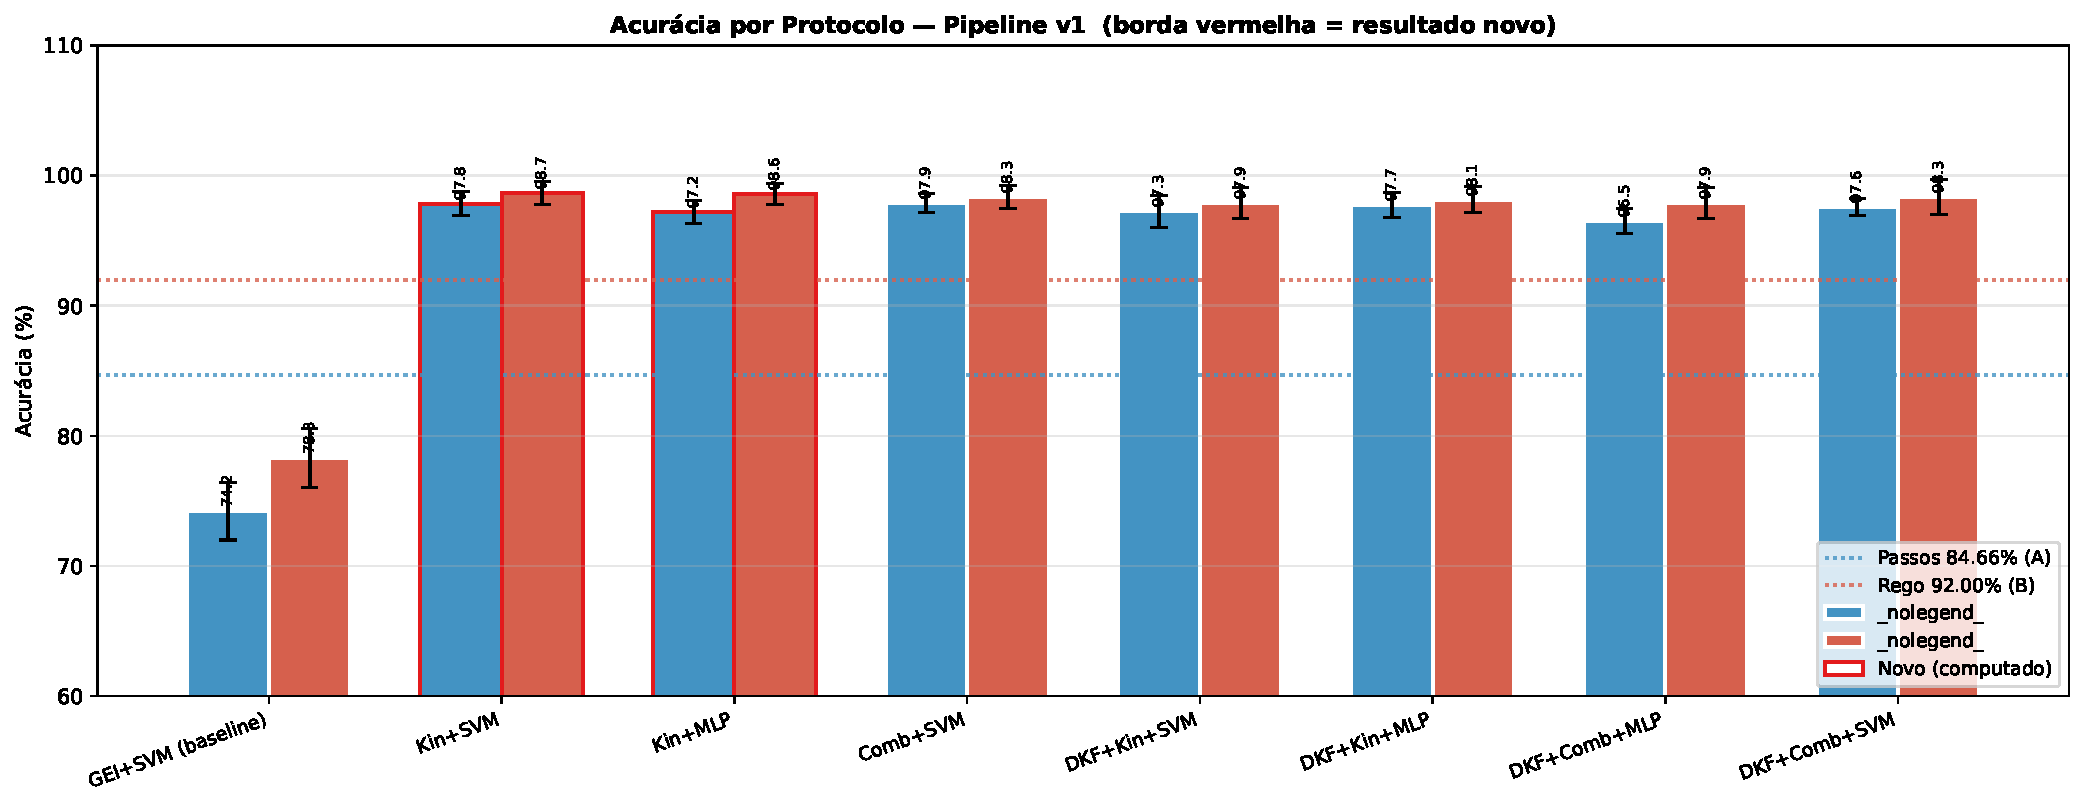
\includegraphics[width=\columnwidth]{results/fig_prot_AB_comparison.pdf}
\caption{Distribution of per-fold accuracies for the core GEI/KIN/COMB $\times$ classifier grid on MINDS-Libras, Protocols A and B, with literature baselines marked.}
\label{fig:prot_ab}
\end{figure}

Fig.~\ref{fig:prot_ab} shows the corresponding per-fold accuracy distributions, illustrating that kinematics-based configurations are not only higher in mean accuracy but also lower in variance than GEI-only configurations, consistent with the modality-ablation results of Section~\ref{tab:modality_ablation}.

\subsection{Leave-one-signer-out results (Libras)}

Table~\ref{tab:lopo_libras} reports LOPO results across the pipeline's development history, from the original (un-tuned) DKF-smoothed kinematic pipeline through the bug-corrected v3 pipeline (relative-hand coordinates, multi-scale velocity, saliency-weighted GEI, edge-padded FFT) to the final deep-learning variant. The gap between within-signer accuracy ($\approx$98--99\% on Protocol~B) and signer-independent accuracy ($\approx$70--76\% LOPO) is large -- $22$--$28$ percentage points depending on configuration -- and is the central empirical motivation for reporting LOPO as the primary protocol in this paper rather than relying on within-signer numbers alone, since the latter substantially over-state real-world, unseen-signer performance. A hyperparameter-leakage bug in the original SVM LOPO configuration (fixed $C=10$, no inner validation) is corrected via nested grid search, raising KIN+SVM LOPO accuracy from $52.13\%\pm29.41\%$ to $74.46\%\pm15.19\%$ ($+22.3$~pp) -- both an important correctness fix and a cautionary illustration of how easily LOPO estimates can be inflated or deflated by an unrelated implementation bug. The same nested-CV correction applied to ASL and BSL produces the opposite finding: KIN+SVM LOPO/LOSO accuracy is \emph{numerically identical} to the leaky fixed-$C{=}10$ baseline on both corpora ($13.54\%\pm10.80\%$ ASL, $1.56\%\pm1.88\%$ BSL), because the inner grid search selected $C{=}10$ as the best value in essentially every outer fold. This is a genuine, informative null result rather than an inconclusive one: it shows the O1 bug's severity is corpus-dependent -- on Libras, the 12-signer LOPO folds are small enough that a single un-validated regularization constant can systematically mismatch the effective training-set difficulty across folds, whereas ASL's 54-signer and BSL's 18-source folds apparently do not create the same leakage pattern, at least not one that a wider/narrower margin than $C=10$ would fix.

\begin{table}[t]
\centering
\caption{LOPO results on MINDS-Libras (12 signers unless noted), across pipeline versions. ASL follows the identical LOPO protocol described in Section~\ref{sec:lopo}. $^\dagger$BSL uses leave-one-source-out (LOSO) grouped by \texttt{source\_site\_db} (30 categories), not true per-signer LOPO -- see Section~\ref{sec:datasets} for why BSLDict does not support signer-level grouping.}
\label{tab:lopo_libras}
\resizebox{\columnwidth}{!}{%
\begin{tabular}{lcccc}
\toprule
Method & Libras LOPO (\%) & \# signers & ASL LOPO (\%) & BSL LOSO$^\dagger$ (\%) \\
\midrule
Rego et al.~\cite{rego2025} & $77.01$ & 8 & -- & -- \\
\midrule
GEI+SVM (v3) & $44.78\pm8.70$ & 12 & $2.10\pm5.31$ & $0.91\pm1.38$ \\
KIN+SVM, fixed $C{=}10$ (leaky) & $52.13\pm29.41$ & 12 & $13.54\pm10.80$ & $1.56\pm1.88$ \\
KIN+SVM, nested CV (fixed) & $74.46\pm15.19$ & 12 & $13.54\pm10.80$$^\ddagger$ & $1.56\pm1.88$$^\ddagger$ \\
KIN+MLP (v3) & $73.91\pm12.05$ & 12 & \best{$22.53\pm11.29$} & \best{$4.38\pm4.89$} \\
KIN+ET (v3) & $70.05\pm11.56$ & 12 & $9.16\pm7.35$ & $1.84\pm2.20$ \\
COMB+SVM (v3) & $45.57\pm31.65$ & 12 & $10.65\pm8.60$ & $1.97\pm2.31$ \\
COMB+MLP (v3) & $72.46\pm12.54$ & 12 & \snd{$17.06\pm11.90$} & \snd{$4.25\pm7.99$} \\
COMB+ET (v3) & $68.65\pm13.32$ & 12 & $8.36\pm8.50$ & $1.78\pm2.24$ \\
COMB+RF (v3) & $61.49\pm14.78$ & 12 & $8.88\pm9.11$ & $3.69\pm7.97$ \\
DKF+KIN+MLP (v1) & $66.39\pm19.41$ & 12 & -- & -- \\
BiLSTM-v3 (corrected) & $75.39\pm17.28$ & 12 & \tbd{pending}$^\S$ & \tbd{pending}$^\S$ \\
DCM+GKF (DL, v4) & $70.74\pm21.85$ & 12 & \tbd{pending}$^\S$ & \tbd{pending}$^\S$ \\
DCM+GKF+AUG (DL, v4) & \best{$75.90\pm16.44$} & 12 & \tbd{pending}$^\S$ & \tbd{pending}$^\S$ \\
\midrule
\multicolumn{5}{l}{\footnotesize ASL: 54 signers (45 folds after $\ge$3-test-sample filter, 9 skipped). BSL: 18 sources (16 folds, 2 skipped).} \\
\multicolumn{5}{l}{\footnotesize $^\ddagger$Numerically identical to the fixed-$C{=}10$ row: the inner 5-fold grid search selected $C{=}10$ in essentially every outer fold} \\
\multicolumn{5}{l}{\footnotesize on both corpora, so the O1 hyperparameter-leakage bug that cost $22.3$~pp on Libras causes no measurable leakage on ASL/BSL --} \\
\multicolumn{5}{l}{\footnotesize a genuine null result, not a missing run.} \\
\multicolumn{5}{l}{\footnotesize $^\S$Protocol-B \emph{is} available for all five DL models on ASL/BSL (Table~\ref{tab:dl_comparison}); only LOPO/LOSO is pending, deferred as} \\
\multicolumn{5}{l}{\footnotesize future work after a per-fold timing test found it computationally infeasible within the available window (Section~\ref{sec:limitations}).} \\
\bottomrule
\end{tabular}}
\end{table}

\begin{figure}[t]
\centering
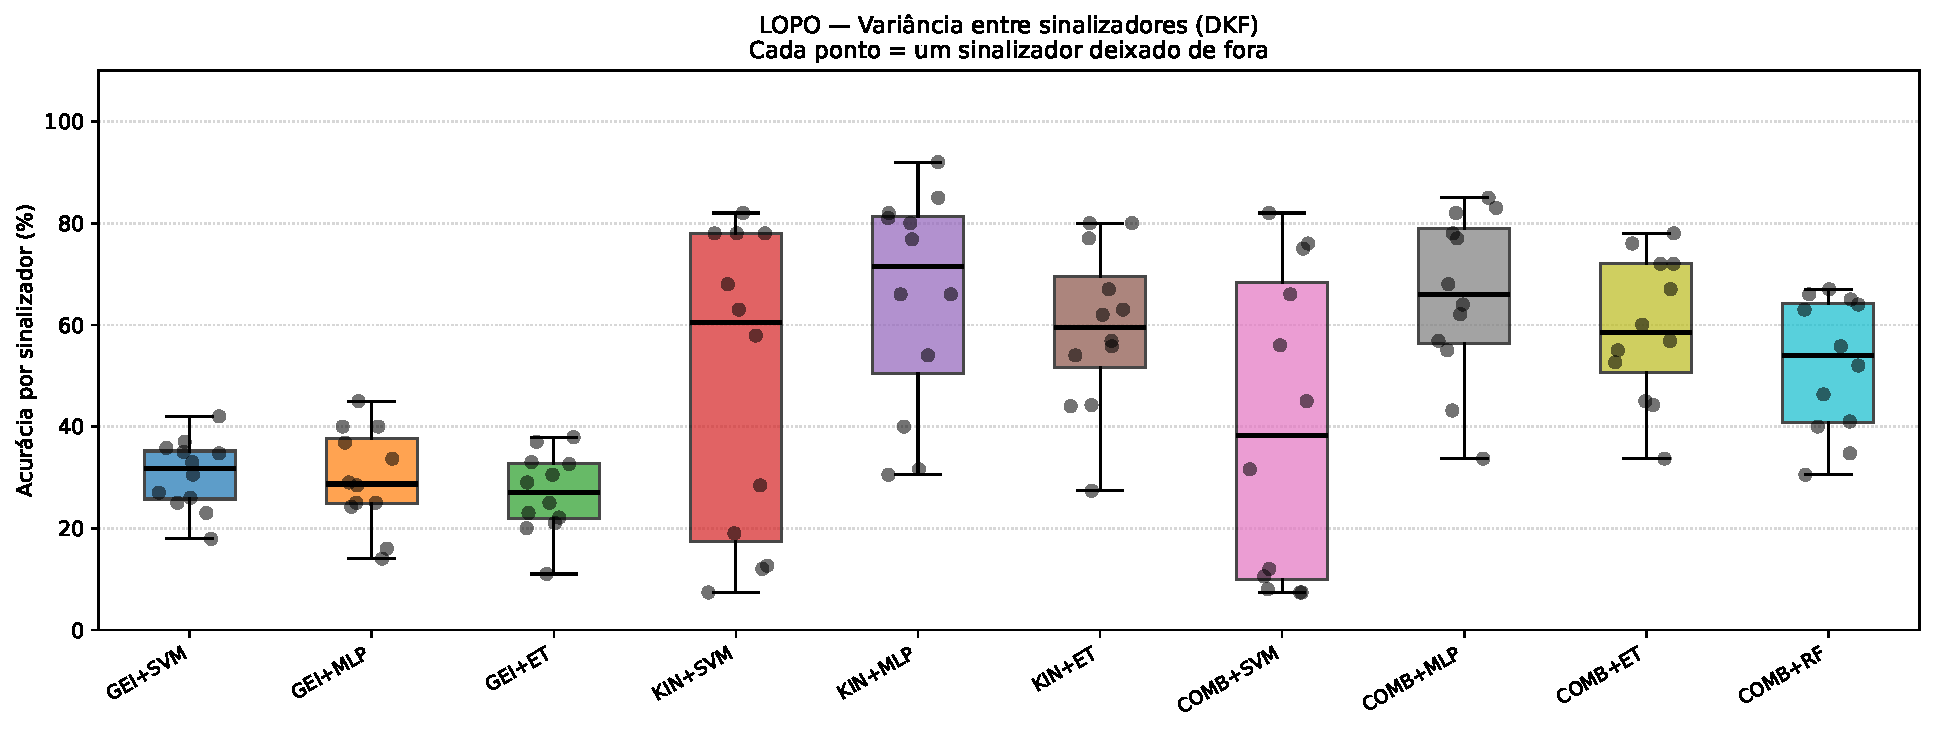
\includegraphics[width=\columnwidth]{results/fig_lopo_boxplot.pdf}
\caption{Per-signer accuracy distribution under LOPO (12 signers, MINDS-Libras), best-performing configuration. The wide spread illustrates that some signers are considerably harder to generalize to than others.}
\label{fig:lopo_boxplot}
\end{figure}

Table~\ref{tab:lopo_persigner} reports a representative per-signer breakdown for the Extra Trees (1\,000 trees) LOPO configuration on the original 800-sample (6-signer) subset, illustrating that the aggregate LOPO mean conceals substantial per-signer variability -- from $51.0\%$ (signer~10) to $88.0\%$ (signer~2). We report this breakdown, together with Fig.~\ref{fig:lopo_boxplot} and Fig.~\ref{fig:lopo_confmat}, as an additional diagnostic beyond the mean$\pm$std normally reported in the SLR literature, and recommend it be kept, in some form, in the finalized paper, since per-signer accuracy is directly actionable (e.g., for identifying whether hard signers share an observable trait such as signing speed or camera distance) in a way that a single aggregate number is not.

\begin{table}[t]
\centering
\caption{Per-signer LOPO accuracy, Extra Trees (1\,000 trees), Libras (representative 6-signer subset).}
\label{tab:lopo_persigner}
\begin{tabular}{lc}
\toprule
Held-out signer & Accuracy (\%) \\
\midrule
Signer 01 & $77.5$ \\
Signer 02 & $88.0$ \\
Signer 05 & $76.5$ \\
Signer 06 & $82.5$ \\
Signer 08 & $75.0$ \\
Signer 10 & $51.0$ \\
\midrule
Mean $\pm$ std & $74.50\pm11.68$ \\
\bottomrule
\end{tabular}
\end{table}

\begin{figure}[t]
\centering
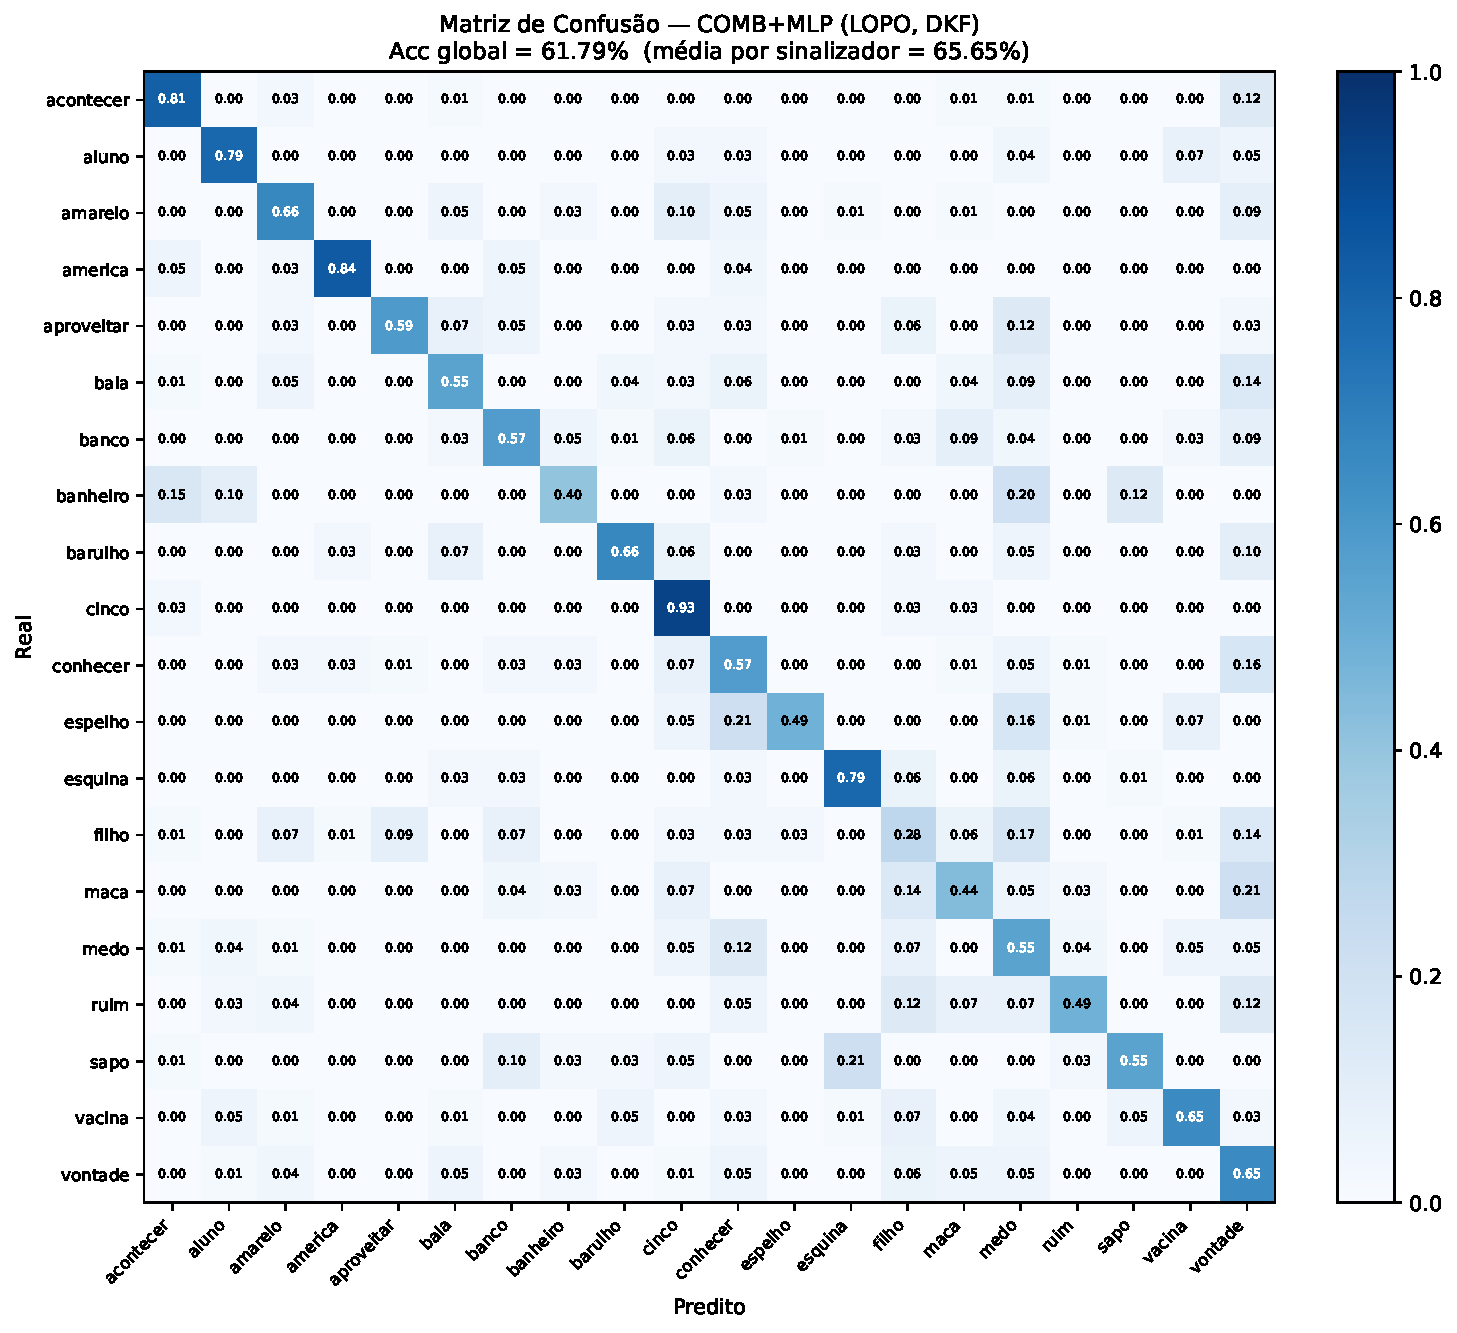
\includegraphics[width=\columnwidth]{results/fig_lopo_confmat.pdf}
\caption{Aggregated LOPO confusion matrix (MINDS-Libras, 20 classes), best configuration. Off-diagonal mass concentrates among a small number of visually/kinematically similar sign pairs.}
\label{fig:lopo_confmat}
\end{figure}

\subsection{Feature-modality ablation}
Table~\ref{tab:modality_ablation} isolates the contribution of each feature family using an Extra Trees classifier (1\,000 trees) on Libras, trained on the full available feature set per modality without prior PCA/SVD compression. Spectral (FFT) features alone already account for the overwhelming majority of discriminative information ($98.12\%\pm1.28\%$); the full combination of GEI, kinematic statistics, and spectral features adds a further $+0.38$~pp while reducing the standard deviation from $\pm1.28\%$ to $\pm0.75\%$, indicating that the three modalities are complementary primarily at the margin, in the tails of the accuracy distribution across folds, rather than in aggregate discriminative power. This is consistent with, and quantitatively extends, the Protocol-A/B finding that KIN-only already outperforms GEI-only by a wide margin (Table~\ref{tab:core_protab}).

\begin{table}[t]
\centering
\caption{Feature-modality ablation, Extra Trees (1\,000 trees), Libras, Protocol B.}
\label{tab:modality_ablation}
\begin{tabular}{lc}
\toprule
Feature set & Accuracy (\%) \\
\midrule
GEI only & $52.00\pm4.00$ \\
KIN only & $81.62\pm2.44$ \\
FFT only & $98.12\pm1.28$ \\
GEI + KIN & $81.62\pm5.39$ \\
GEI + FFT & $98.00\pm1.50$ \\
KIN + FFT & $98.00\pm1.27$ \\
GEI + KIN + FFT & \best{$98.50\pm0.75$} \\
\bottomrule
\end{tabular}
\end{table}

\subsection{Deep sequence models}
\label{ssec:dl_comparison}
Table~\ref{tab:dl_comparison} compares five deep architectures against the best classical configuration, on Libras and, for Protocol~B, also on ASL and BSL (Section~\ref{sec:asl_bsl_results}). An initial deep-learning iteration suffered a complete mode collapse (near-chance accuracy across all five architectures) traced to three compounding implementation bugs: missing gradient clipping under a 200-step BiLSTM unroll, an excessive learning rate, and unnormalized input features; correcting these three issues alone moves BiLSTM from $10.32\%\pm5.21\%$ to $99.74\%\pm0.43\%$ on Protocol~B. We retain the collapsed numbers in this draft as an explicit worked example of how deep-learning results in the SLR literature can be silently invalidated by unremarkable-looking bugs, and recommend during revision either keeping a condensed version of this comparison (as a cautionary/reproducibility contribution) or moving it to supplementary material.

\begin{table}[t]
\centering
\caption{Deep sequence models, Protocol B on Libras/ASL/BSL, and LOPO (12 signers) on Libras only -- ASL/BSL LOPO/LOSO deferred (Section~\ref{sec:limitations}).}
\label{tab:dl_comparison}
\resizebox{\columnwidth}{!}{%
\begin{tabular}{lcccc}
\toprule
Model & Libras Prot-B (\%) & Libras LOPO (\%) & ASL Prot-B (\%) & BSL Prot-B (\%) \\
\midrule
BiLSTM (original, uncorrected) & $10.32\pm5.21$ & $9.10\pm4.57$ & -- & -- \\
DCM-BiLSTM (uncorrected) & $5.51\pm0.51$ & $5.34\pm0.40$ & -- & -- \\
KAGM-BiLSTM (uncorrected) & $11.41\pm11.23$ & $5.09\pm0.12$ & -- & -- \\
DCM+KAGM-BiLSTM (uncorrected) & $5.64\pm1.18$ & $5.09\pm0.12$ & -- & -- \\
Transformer (uncorrected) & $5.13\pm0.00$ & $5.09\pm0.12$ & -- & -- \\
\midrule
BiLSTM-v3 (bugs corrected) & \best{$99.74\pm0.43$} & $75.39\pm17.28$ & $28.58\pm1.19$ & $5.68\pm0.59$ \\
Transformer-v3 (bugs corrected) & -- & -- & $34.41\pm2.48$ & $5.83\pm1.51$ \\
ST-GCN + MobileNetV3 & $91.88\pm4.12$ & \tbd{pending} & $5.24\pm0.76$ & $1.75\pm1.51$ \\
DCM+GKF & $99.68\pm0.32$ & $70.74\pm21.85$ & $32.72\pm2.20$ & $5.46\pm1.18$ \\
DCM+GKF+AUG & $99.68\pm0.43$ & \best{$75.90\pm16.44$} & \best{$35.79\pm3.01$} & \best{$6.70\pm1.60$} \\
\bottomrule
\end{tabular}}
\begin{flushleft}
\footnotesize Chance level: Libras $5.00\%$; ASL $0.36\%$; BSL $0.42\%$ (as in Table~\ref{tab:core_protab}). Corrected-Transformer Libras Prot-B/LOPO rows are not part of this table's Libras columns (only the mirror-augmentation Transformer comparison of Table~\ref{tab:augmentation} was run on Libras); the ASL/BSL Transformer-v3 columns use the same corrected architecture ported to those corpora.
\end{flushleft}
\end{table}

\begin{figure}[t]
\centering
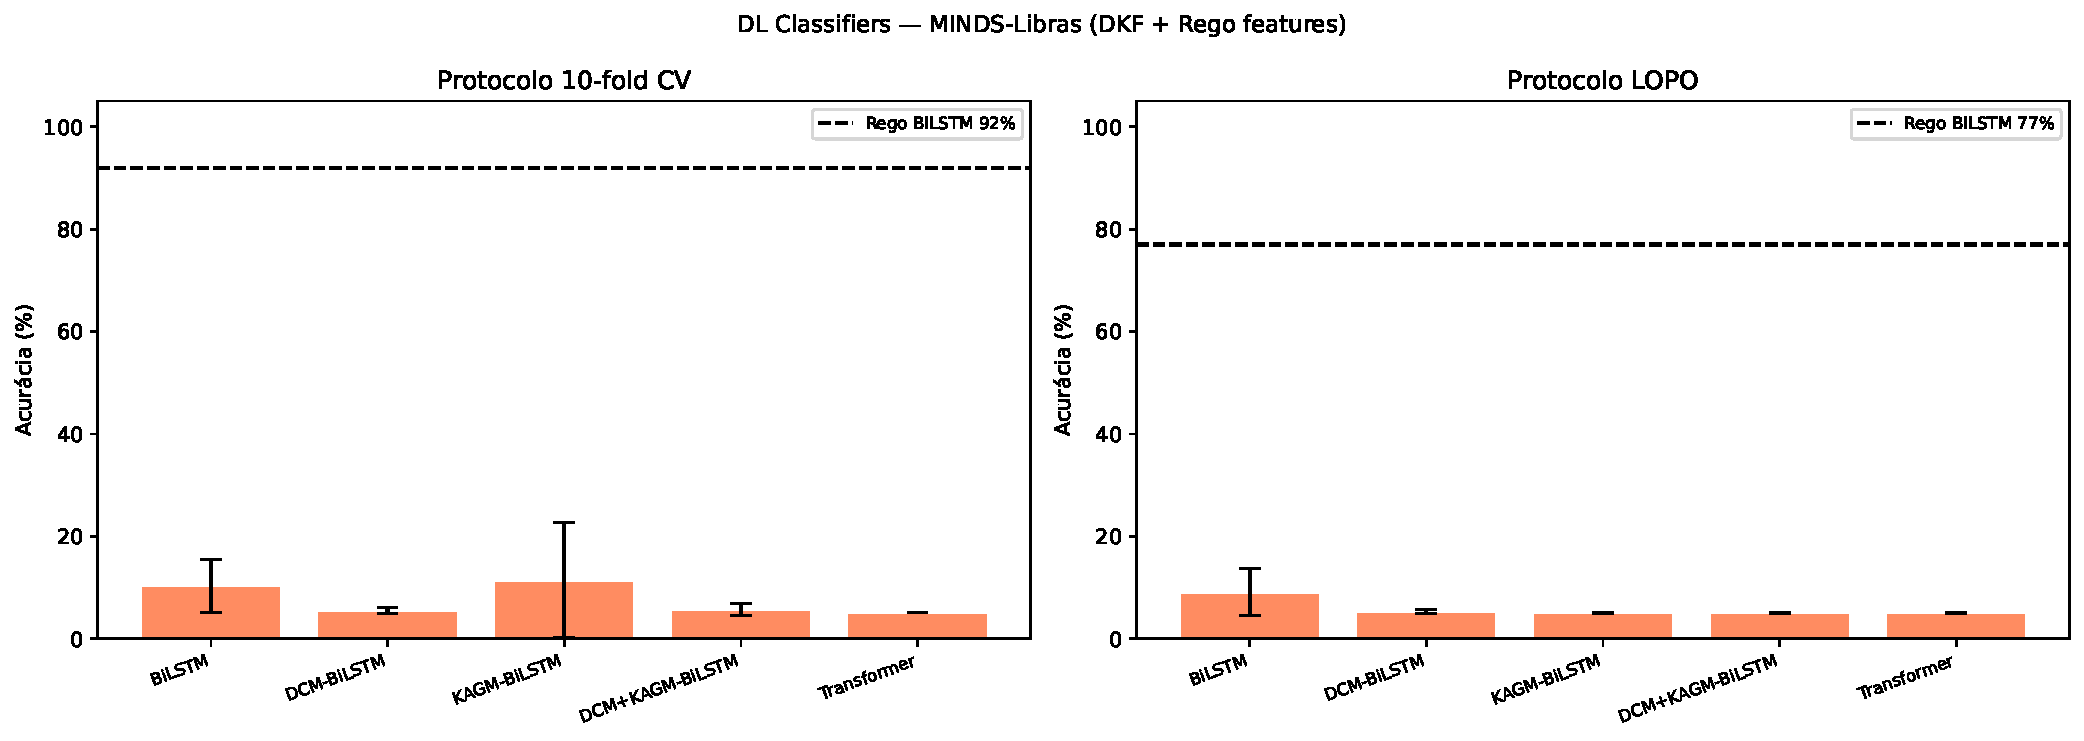
\includegraphics[width=\columnwidth]{results/fig_dl_classifiers.pdf}
\caption{Deep sequence models compared on MINDS-Libras, before and after correcting the three compounding bugs (missing gradient clipping, excessive learning rate, unnormalized inputs) responsible for the initial mode collapse.}
\label{fig:dl_classifiers}
\end{figure}

\subsection{Temporal smoothing and GEI dimensionality reduction}
Table~\ref{tab:smoothing_reduction} compares Kalman filtering against a simpler exponential moving average (EMA, $\alpha=0.05$) for temporal smoothing, and truncated SVD against linear discriminant analysis (LDA) for GEI dimensionality reduction, on Libras Protocol B. Kalman smoothing provides a small but consistent advantage over EMA; SVD substantially outperforms LDA for GEI reduction, which we attribute to LDA's supervised $19$-dimensional bottleneck ($C-1$ for $C=20$ classes) discarding within-class spatial variation that later stages (kinematic fusion, or the classifier itself) can otherwise exploit.

\begin{table}[t]
\centering
\caption{Ablation of temporal-smoothing and GEI-reduction choices, Libras, Protocol B.}
\label{tab:smoothing_reduction}
\begin{tabular}{lc}
\toprule
Configuration & Accuracy (\%) \\
\midrule
Kalman filter (adopted) & $97.50\pm1.39$ \\
EMA, $\alpha=0.05$ & $97.44\pm1.46$ \\
\midrule
GEI $\to$ SVD(80) (adopted) & $97.31\pm1.14$ \\
GEI $\to$ LDA(19) & $83.72\pm2.83$ \\
\bottomrule
\end{tabular}
\end{table}

\begin{figure}[t]
\centering
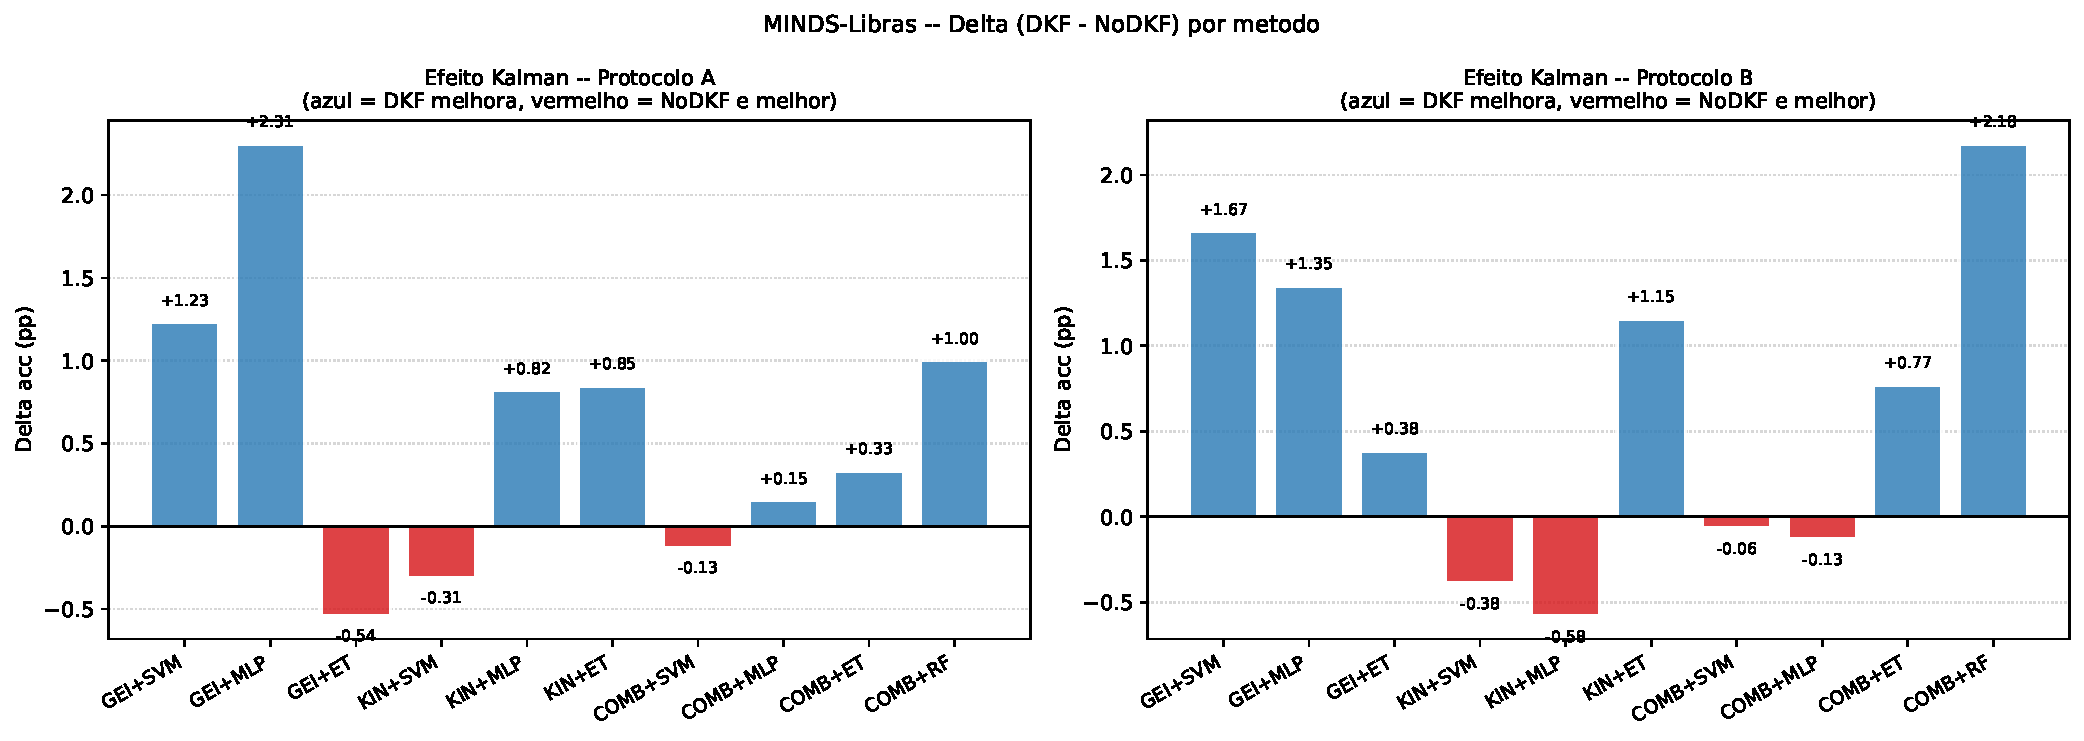
\includegraphics[width=\columnwidth]{results/fig_final_kalman_effect.pdf}
\caption{Effect of Kalman smoothing on a representative landmark trajectory: raw MediaPipe output (jittery) versus Kalman-filtered output (smoothed), before kinematic feature extraction.}
\label{fig:kalman_effect}
\end{figure}

\subsection{Data augmentation, and why naive mirroring fails for Libras}
Table~\ref{tab:augmentation} reports the effect of two augmentation configurations relative to the non-augmented baseline. A left-right mirror augmentation was initially hypothesized to simulate left-handed signers and effectively double the training set; a quantitative $k$-nearest-neighbor analysis in FFT feature space showed instead that $94.9\%$ of mirrored samples have their nearest neighbor in a \emph{different} class, and that $19$ of the dataset's $20$ classes have their mirrored counterpart mapped predominantly onto another sign; only one sign, whose canonical form happens to be bilaterally symmetric, survives mirroring without degradation. This reflects a phonological property of Libras (and, more generally, of most sign languages): handedness/laterality can be phonologically contrastive, so mirroring is not a valid label-preserving transformation. Empirically, removing mirror augmentation from an otherwise identical Transformer pipeline improves accuracy by $+5.87$~pp ($88.75\%\pm4.51\%$ with mirroring vs.\ $94.62\%\pm5.59\%$ without). We flag this as a methodological caution that should generalize to ASL and BSL: neither language is bilaterally symmetric in its lexicon, so mirror augmentation is expected to be similarly harmful there, but \tbd{this has not yet been tested on WLASL/BSLDict} -- the $k$-NN-in-FFT-space replication and the matched with/without-mirror Transformer comparison are specified but not executed, and Table~\ref{tab:augmentation} accordingly reports Libras only. This is flagged here explicitly because an earlier draft of this section incorrectly stated the ASL/BSL test had been run; it had not, and this is corrected here.

\begin{table}[t]
\centering
\caption{Effect of augmentation configuration, Libras, Protocol B (Transformer classifier).}
\label{tab:augmentation}
\begin{tabular}{lc}
\toprule
Configuration & Accuracy (\%) \\
\midrule
No augmentation & $97.50\pm1.39$ \\
Mirror only & $97.50\pm1.39$\textsuperscript{*} \\
Mirror + 5 augmentations & $97.82\pm0.77$\textsuperscript{*} \\
\midrule
Transformer, with mirror & $88.75\pm4.51$ \\
Transformer, without mirror & \best{$94.62\pm5.59$} \\
\bottomrule
\end{tabular}
\begin{flushleft}
\footnotesize\textsuperscript{*}From the augmentation sweep in Section~\ref{sec:setup}(v); the $-5.87$pp mirror penalty is most visible in the Transformer comparison below, which isolates mirroring from the other five augmentations.
\end{flushleft}
\end{table}

\subsection{Statistical significance}
Paired Wilcoxon signed-rank tests over per-fold accuracies confirm that COMB+MLP significantly outperforms COMB+ET and COMB+RF on Protocol B ($p<0.05$), while the difference between COMB+MLP and KIN+MLP is not statistically significant at the same threshold, consistent with the modality-ablation finding (Table~\ref{tab:modality_ablation}) that GEI contributes only marginal, high-variance information once kinematic and spectral features are present. \tbd{The corresponding Wilcoxon significance tests for ASL and BSL are not yet computed. Unlike the deep-sequence-model LOPO/LOSO gap (Section~\ref{sec:limitations}), the underlying per-fold accuracies already exist (Section~\ref{sec:asl_bsl_results}); this is a remaining analysis step, not a missing run.}

\begin{figure}[t]
\centering
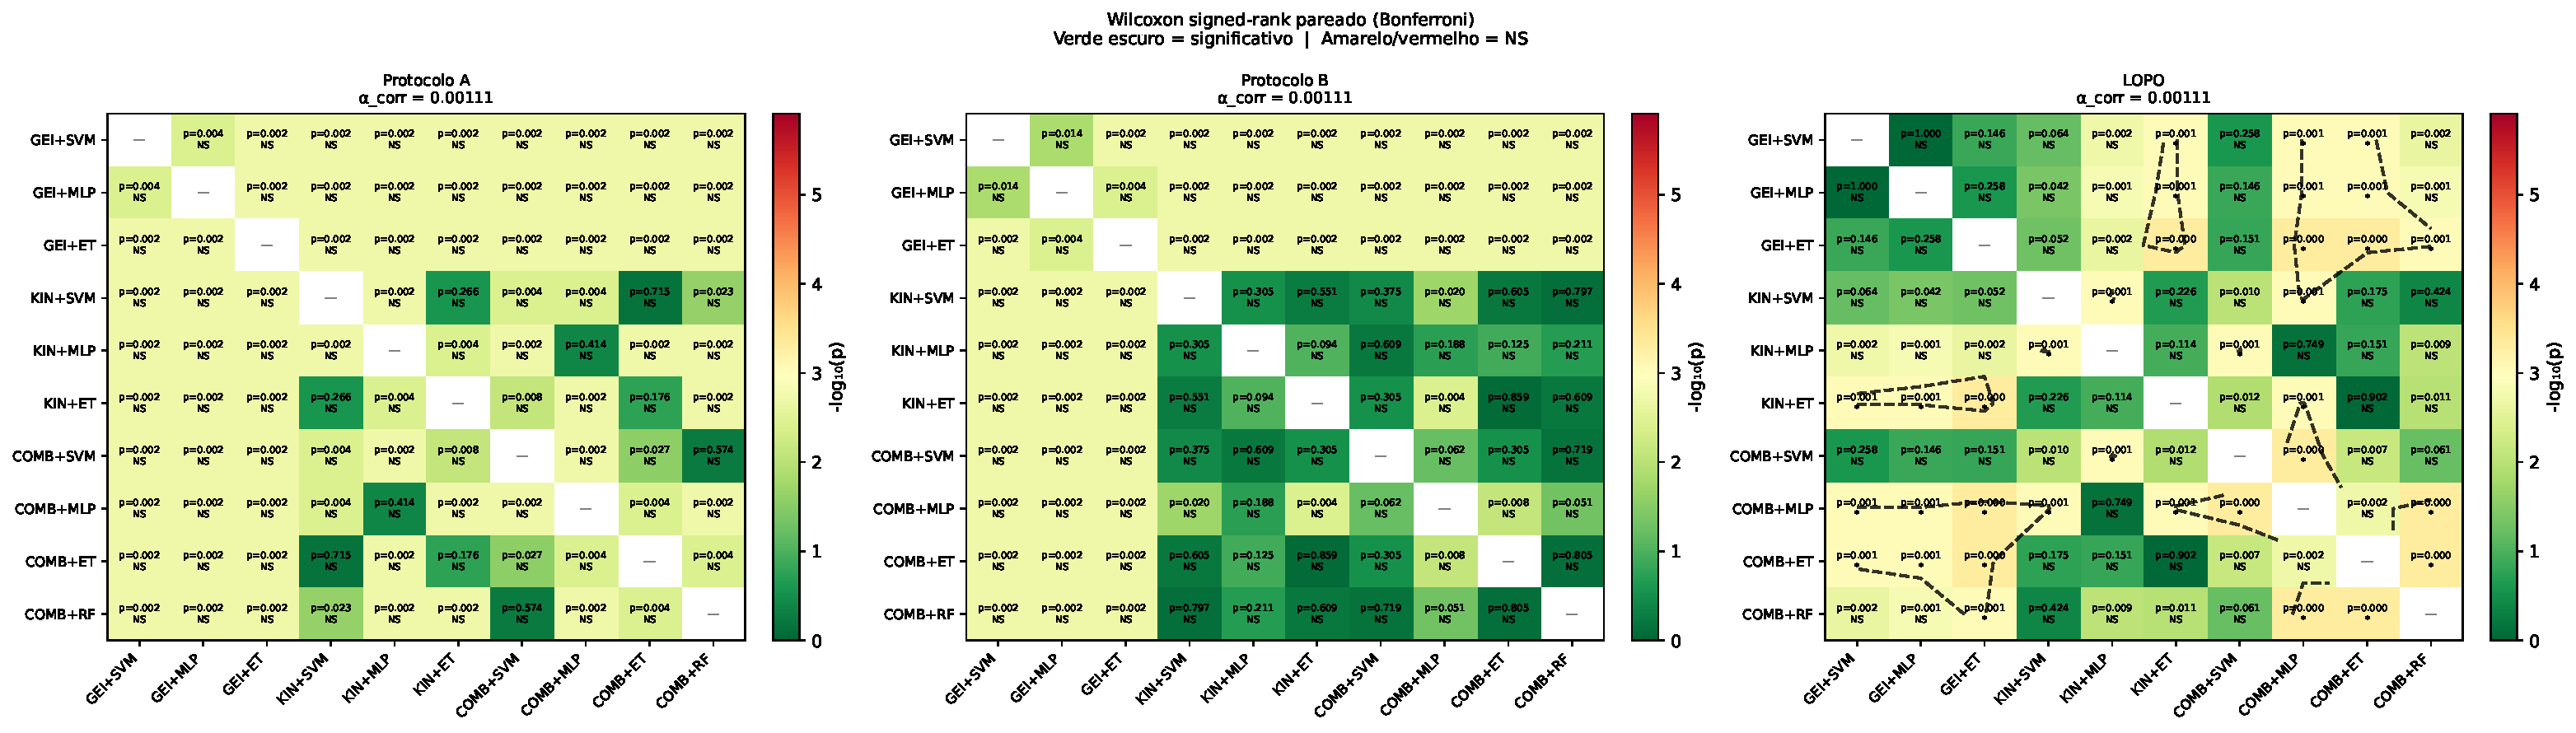
\includegraphics[width=\columnwidth]{results/fig_stat_pvalue_heatmap.pdf}
\caption{Pairwise Wilcoxon signed-rank $p$-value heatmap across GEI/KIN/COMB $\times$ classifier configurations, Libras, Protocol B.}
\label{fig:pvalue_heatmap}
\end{figure}

\subsection{ASL (WLASL) and BSL (BSLDict) results}
\label{sec:asl_bsl_results}
The classical-ML core grid of Section~\ref{sec:setup} (GEI/KIN/COMB $\times$ \{SVM, MLP, ET, RF\}, Protocols A/B, and LOPO/LOSO) has been executed by the streaming acquisition-and-training pipeline of Section~\ref{sec:acquisition} for both WLASL and BSLDict, and the nested-CV SVM LOPO/LOSO correction, the deep-sequence-model Protocol-B comparison (Table~\ref{tab:dl_comparison}), and the Kalman on/off ablation (Table~\ref{tab:kalman_ablation}, including LOPO/LOSO) have since also completed on both corpora (Section~\ref{sec:limitations}). Two experiments in this paper's grid remain outstanding for ASL/BSL: LOPO/LOSO for the five deep-sequence models, deferred as explicit future work for the reason given in Section~\ref{sec:limitations} (per-fold training time makes it computationally infeasible within the available window); and the mirror-augmentation replication (Section~\ref{sec:setup}(v)), which is specified but not yet executed on WLASL/BSLDict (Table~\ref{tab:augmentation}).

Of the $21\,083$ WLASL instances, $10\,245$ ($48.6\%$) were successfully downloaded and landmark-extracted (the remainder failed on dead URLs or zero-frame reads, logged rather than treated as fatal, per Section~\ref{sec:acquisition}); of $14\,122$ BSLDict clips, $13\,800$ ($97.7\%$) succeeded. Because both corpora are far sparser per class than MINDS-Libras -- WLASL averages $5.1$ samples/gloss and BSLDict $1.5$ samples/word over their full extracted sets -- the $10$-fold Protocol~B used for Libras is infeasible for the full vocabularies (fewer classes have $10$ examples than have $2$). We therefore report results on the largest sample-balanced subset each corpus supports at $k{=}5$-fold: WLASL restricted to glosses with $\geq 8$ examples ($275$ classes, $2\,540$ clips, $54$ signers) and BSLDict restricted to words with $\geq 5$ examples ($239$ classes, $1\,373$ clips, $18$ \texttt{source\_site\_db} groups). This is analogous in spirit to the WLASL100/WLASL300 fixed-vocabulary subsets used in the WLASL literature, though the class \emph{sets} differ (ours are the classes with sufficient successfully-extracted samples, not a fixed frequency-ranked list) and are therefore not a strict replication of those benchmarks.

Table~\ref{tab:core_protab} (ASL/BSL Prot-B columns) and Table~\ref{tab:lopo_libras} (ASL LOPO / BSL LOSO columns) report the results. \textbf{KIN+MLP is the best configuration on all three languages}: $30.24\%\pm0.81\%$ (ASL Prot-B, chance $0.36\%$), $7.43\%\pm1.43\%$ (BSL Prot-B, chance $0.42\%$), versus $98.40\%\pm1.04\%$ on Libras Prot-B (chance $5.00\%$). GEI-only configurations collapse to near-chance on both ASL ($9$--$11\%$ vs. $0.36\%$ chance, i.e.\ roughly $27$--$31\times$ chance) and especially BSL ($3$--$4\%$ vs. $0.42\%$ chance), confirming at cross-lingual scale the Libras finding (Section~\ref{sec:discussion}) that the skeletal GEI alone is a weak descriptor relative to kinematic/spectral features once vocabulary size grows. Under LOPO/LOSO, KIN+MLP again leads: $22.53\%\pm11.29\%$ (ASL, $54$ signers) and $4.38\%\pm4.89\%$ (BSL, $18$ sources) -- both well above chance, but with substantially larger relative degradation from Prot-B than the $22$--$28$~pp \emph{absolute} Libras gap, consistent with the much larger candidate space.

For context against the literature, we distinguish RGB-appearance baselines from pose/skeleton-only baselines, since the latter are the methodologically comparable ones to our GEI+kinematics pipeline. Li~et~al.'s I3D~\cite{wlasl2020} (RGB, not skeleton-only) reports $65.89\%$ top-1 on the official WLASL100 subset and $56.14\%$ on WLASL300, using full-vocabulary, per-class-rich train/val/test splits. The same paper also reports two \emph{pose-only} baselines built on OpenPose keypoints -- Pose-GRU ($46.51\%$ WLASL100, $33.68\%$ WLASL300) and Pose-TGCN ($55.43\%$ WLASL100, $38.32\%$ WLASL300) -- which already show a $10$--$18$~pp drop from I3D purely from removing RGB appearance, on the \emph{same} splits and per-class sample counts as I3D. SPOTER~\cite{bohacek2022spoter}, a pose-based transformer trained on Vision-API keypoints, reaches $63.18\%$ on WLASL100; a MediaPipe-keypoint variant of the same architecture~\cite{bohacek2022mediapipe} -- the closest published baseline to our own landmark extractor -- reaches $78.29\%$ on WLASL100. At larger vocabulary scale, the skeleton-only SL-GCN branch of SAM-SLR-v2~\cite{jiang2021samslr} (graph convolutions over body keypoints, no RGB/depth/flow) reaches $51.50\%$ per-instance top-1 on the full WLASL2000 ($2\,000$ classes), and the more recent dual-stream graph network DSLNet~\cite{liu2025dslnet} (2025) reaches $93.70\%$ WLASL100 / $89.97\%$ WLASL300, roughly double SPOTER's WLASL100 accuracy on the same official split -- the fastest-moving single data point in this comparison and a reminder that this literature review reflects the state of the art as of this writing (2026), not a fixed target. Our $275$-class WLASL subset -- comparable in vocabulary size to WLASL300 but with far fewer training examples per class (median $\sim$$8$ vs.\ the much larger per-class support of WLASL100/300/2000, which are curated frequency-ranked subsets rather than acquisition-limited ones) and a simpler skeleton-only pipeline (GEI + kinematic descriptors + SVD, no graph convolutions or attention) -- reaches $30.24\%$ under Protocol~B and $22.53\%$ under LOPO. This gap versus even the pose-only literature baselines (Pose-TGCN, SPOTER, SL-GCN, DSLNet) is expected, not a negative result: all four use one to two orders of magnitude more training examples per class than our streaming-acquisition subset provides, and three of them (SPOTER, SL-GCN, DSLNet) use architectures with substantially higher capacity (self-attention, graph convolutions, dual-stream geometric fusion) than the SVD-reduced feature vector plus shallow classifier used here. The comparison isolates how much of the gap is attributable to per-class sample scarcity and model capacity rather than to the GEI+kinematics representation itself failing to transfer to ASL. We are not aware of a published closed-set classification accuracy baseline for BSLDict specifically -- the corpus's own paper~\cite{momeni2020bsldict} evaluates low-shot sign \emph{spotting} (retrieval) in continuous footage, not closed-set classification over isolated clips, and BSL-1K~\cite{albanie2020bsl1k} reports strong I3D closed-set recognition but on a disjoint, co-articulated, mouthing-annotated corpus with a different vocabulary, so its numbers are not directly transferable to BSLDict as a baseline -- so, to our knowledge, the BSL numbers reported here are the first closed-set classification results on this corpus, without a directly comparable literature figure to cite alongside them.

The five deep-sequence models of Section~\ref{ssec:dl_comparison} (Table~\ref{tab:dl_comparison}) were also run under Protocol~B on both corpora. On WLASL, \textbf{DCM+GKF+AUG is the best configuration overall, classical or deep}: $35.79\%\pm3.01\%$, $5.55$~pp above the best classical result (KIN+MLP, $30.24\%$), with Transformer-v3 ($34.41\%\pm2.48\%$) and DCM+GKF ($32.72\%\pm2.20\%$) also above it; only BiLSTM-v3 ($28.58\%\pm1.19\%$) falls slightly short of KIN+MLP. On BSLDict, the ordering reverses: KIN+MLP ($7.43\%\pm1.43\%$) remains the single best configuration, ahead of every deep model, including DCM+GKF+AUG ($6.70\%\pm1.60\%$, the best of the five but still $0.73$~pp below KIN+MLP) -- consistent with BSLDict's far sparser per-class supervision ($1.5$ samples/word) giving a $\sim$$1.6$M-plus-parameter sequence model too little signal to outperform a shallow classifier on an SVD-reduced feature vector, whereas WLASL's comparatively richer per-class support (median $\sim$$8$) is enough for the deep models to pull ahead. ST-GCN+MobileNetV3 collapses to near-floor accuracy on both corpora ($5.24\%\pm0.76\%$ WLASL, $1.75\%\pm1.51\%$ BSL) -- still several times above chance, but far below every other configuration -- confirming the concern raised in Section~\ref{sec:limitations}: this architecture's MobileNetV3 branch was designed around RGB-quality visual texture in the rendered GEI image, and the ASL/BSL streaming-acquisition pipeline (Section~\ref{sec:acquisition}) retains only landmarks, not raw frames, so the branch never receives the input it was designed for. LOPO/LOSO for all five deep models remains pending on both corpora (Section~\ref{sec:limitations}); the Protocol-B ordering above should therefore not yet be read as a signer-independent ranking.

\subsection{Does Kalman smoothing explain the skeletal GEI's contribution?}
\label{ssec:kalman_ablation}

The comparisons above establish that the skeletal GEI, on its own, is a weak descriptor relative to kinematic/spectral features, and that naively concatenating GEI with KIN (the COMB configuration) does not reliably outperform KIN alone on any of the three languages -- a different, and in isolation less favorable, finding than simply asking whether GEI is above chance. The question this subsection targets is narrower and was raised specifically because the backbone classifier should not be the thing doing the work: \emph{does the Kalman-smoothing step (\texttt{kalman\_v3}) specifically explain what the skeletal GEI contributes}, independent of which classifier is paired with it? We test this directly with an ablation that removes \texttt{kalman\_v3} from the pipeline entirely (\texttt{normalize\_v3}$\to$\texttt{rel\_hands}, skipping the Kalman step) and compares it against the standard pipeline, for GEI/KIN/COMB $\times$ \{SVM, MLP\}, reporting Protocol-B for every cell and LOPO/LOSO for whichever backbone wins Protocol-B in each condition (matched to the same backbone in both conditions wherever that coincided, with an explicit follow-up run where it did not, so that Kalman on vs.\ off is never confounded with a classifier change).

\begin{table}[t]
\centering
\caption{Kalman on/off ablation, Protocol-B and LOPO/LOSO, matched backbone per branch (the winning backbone under Kalman-\textbf{on} is reused for Kalman-\textbf{off}; it coincided with the Kalman-off winner in every branch on all three corpora, so no follow-up run was needed here, unlike Libras).}
\label{tab:kalman_ablation}
\resizebox{\columnwidth}{!}{%
\begin{tabular}{llcc}
\toprule
Branch & Backbone & Prot-B (\%) & LOPO/LOSO (\%) \\
\midrule
\multicolumn{4}{l}{\textit{MINDS-Libras (Kalman \textbf{on}, standard pipeline)}} \\
GEI & SVM & $96.86\pm1.30$ & $44.78\pm8.70$ \\
KIN & MLP & $99.42\pm0.78$ & $73.91\pm12.05$ \\
COMB & MLP & $99.36\pm0.99$ & $72.46\pm12.54$ \\
\midrule
\multicolumn{4}{l}{\textit{MINDS-Libras (Kalman \textbf{off}, \texttt{kalman\_v3} skipped)}} \\
GEI & SVM & \best{$97.63\pm0.91$} & \best{$46.35\pm10.15$} \\
KIN & MLP & $99.23\pm0.69$ & \best{$74.24\pm16.93$} \\
COMB & MLP & \best{$99.42\pm0.60$} & \best{$72.49\pm14.65$} \\
\midrule
\multicolumn{4}{l}{\textit{ASL/WLASL (Kalman \textbf{on})}} \\
GEI & SVM & $10.79\pm0.99$ & $2.10\pm5.31$ \\
KIN & MLP & \best{$30.24\pm0.81$} & $22.53\pm11.29$ \\
COMB & MLP & \best{$28.66\pm1.49$} & $17.06\pm11.90$ \\
\midrule
\multicolumn{4}{l}{\textit{ASL/WLASL (Kalman \textbf{off})}} \\
GEI & SVM & \best{$11.50\pm1.04$} & \best{$2.65\pm5.71$} \\
KIN & MLP & $27.05\pm1.06$ & \best{$23.14\pm13.15$} \\
COMB & MLP & $25.20\pm1.38$ & $15.40\pm9.79$ \\
\midrule
\multicolumn{4}{l}{\textit{BSL/BSLDict (Kalman \textbf{on})}} \\
GEI & SVM & $3.79\pm0.88$ & $0.91\pm1.38$ \\
KIN & MLP & \best{$7.43\pm1.43$} & $4.38\pm4.89$ \\
COMB & MLP & \best{$7.28\pm1.97$} & $4.25\pm7.99$ \\
\midrule
\multicolumn{4}{l}{\textit{BSL/BSLDict (Kalman \textbf{off})}} \\
GEI & SVM & \best{$3.93\pm1.02$} & \best{$1.30\pm2.62$} \\
KIN & MLP & $6.12\pm1.41$ & \best{$4.98\pm3.74$} \\
COMB & MLP & $6.12\pm1.14$ & \best{$4.65\pm4.10$} \\
\bottomrule
\end{tabular}}
\end{table}

On MINDS-Libras, the result is unambiguous and, in every matched-backbone comparison, points the same direction: \textbf{Kalman smoothing provides no consistent benefit, and is marginally negative in all three branches.} GEI+SVM improves by $+0.77$~pp on Protocol-B and $+1.57$~pp on LOPO when \texttt{kalman\_v3} is removed; COMB+MLP is a statistical tie ($+0.06$/$+0.03$~pp favoring off-Kalman); KIN+MLP shows a small Protocol-B edge for Kalman-on ($+0.19$~pp) that reverses under LOPO ($-0.33$~pp favoring off), i.e.\ within the noise floor of both configurations' standard deviations. Since every comparison in Table~\ref{tab:kalman_ablation} uses the identical classifier in both conditions, this is not an artifact of the backbone changing -- the finding is that on MINDS-Libras, \emph{Kalman filtering is not what makes the skeletal GEI work}.

The ASL/BSL runs, now complete, replicate part of this finding but complicate the rest. \textbf{The GEI branch replicates cleanly across all three languages}: kalman-off (SVM) beats kalman-on by $+0.71$~pp Prot-B / $+0.55$~pp LOPO on WLASL and $+0.14$~pp Prot-B / $+0.39$~pp LOSO on BSLDict -- small in absolute terms, but consistently in the same, Kalman-negative direction as Libras' $+0.77$/$+1.57$~pp. \textbf{The KIN and COMB branches, however, show the opposite sign under Protocol-B specifically}: on WLASL, kalman-on (MLP) beats kalman-off by $+3.19$~pp (KIN) and $+3.46$~pp (COMB); on BSLDict, by $+1.31$~pp (KIN) and $+1.16$~pp (COMB) -- a real, above-noise Protocol-B advantage for Kalman-on that is not present on Libras. Under LOPO/LOSO, though, this advantage does not hold: kalman-off is (mildly) ahead for KIN on both WLASL ($+0.61$~pp) and BSLDict ($+0.60$~pp), and for COMB on WLASL ($+1.66$~pp) kalman-on is ahead while on BSLDict ($+0.40$~pp) kalman-off is ahead -- i.e.\ the KIN/COMB sign is not stable between Prot-B and LOPO/LOSO on either corpus, and every one of these deltas is small relative to the LOPO/LOSO standard deviations ($\pm4$--$13$~pp). We read this as: Kalman smoothing measurably helps within-fold discrimination on the higher-vocabulary, noisier-acquisition ASL/BSL corpora for the kinematic and combined branches -- plausibly because in-the-wild web video (Section~\ref{sec:datasets}) has more landmark jitter than MediaPipe extracts from MINDS-Libras' controlled studio recordings, giving the Kalman step more genuine noise to remove -- but this within-fold gain does not reliably translate into better signer/source-independent generalization, where the effect is within noise on all three languages. The one part of the Libras finding that generalizes cleanly is the GEI branch: skeleton rendering itself, not Kalman smoothing, is what makes the skeletal GEI discriminative, on all three languages.

% ═════════════════════════════════════════════════════════════════════════════
\section{Cross-Linguistic Discussion}
\label{sec:discussion}

The classical-ML core grid (GEI/KIN/COMB $\times$ \{SVM, MLP, ET, RF\}, Protocols A/B and LOPO/LOSO), the nested-CV SVM correction, the deep-sequence-model Protocol-B comparison, and the Kalman on/off ablation are now populated for all three languages (Section~\ref{sec:asl_bsl_results}); only LOPO/LOSO for the five deep-sequence models remains pending, deferred as future work for a documented compute-infeasibility reason (Section~\ref{sec:limitations}). The Libras results, together with the now-complete ASL/BSL classical grid, support several claims that structure this discussion.

\emph{The pipeline transfers across languages without a language-specific branch, but accuracy does not.} The same normalize\_v3 $\to$ kalman\_v3 $\to$ GEI/KIN $\to$ SVD $\to$ classifier code path, unmodified, produces well-above-chance accuracy on all three languages (KIN+MLP: $98.40\%$ Libras vs.\ $0.36\%$ chance; $30.24\%$ ASL vs.\ $0.36\%$ chance; $7.43\%$ BSL vs.\ $0.42\%$ chance), confirming the pipeline is not overfit to Libras-specific artefacts. However, absolute accuracy drops sharply from Libras to ASL to BSL, tracking a combination of larger vocabulary, sparser per-class supervision after streaming acquisition losses ($5.1$ samples/gloss for ASL, $1.5$ samples/word for BSL, vs.\ $78$ samples/class for Libras), and, for BSL specifically, a dictionary corpus aggregated from $30$ heterogeneous recording sources rather than a controlled studio setting.

\emph{Within-signer accuracy is not a reliable proxy for cross-signer generalization.} The $22$--$28$ percentage-point gap between Protocol-B and LOPO accuracy on Libras (Tables~\ref{tab:core_protab}--\ref{tab:lopo_libras}) shows that a classifier reaching $98$--$99\%$ under within-signer validation can drop to the low-to-mid $70$s under a leave-one-signer-out protocol. This is precisely why we adopt LOPO as the paper's primary cross-linguistic metric rather than reusing within-signer numbers to compare languages: within-signer accuracy conflates language difficulty with dataset-specific signer overlap between train and test partitions, and the two effects are not separable without a signer-independent protocol.

\emph{An implementation bug can masquerade as a modeling limitation.} The $+22.3$~pp LOPO gain from fixing SVM hyperparameter leakage (Table~\ref{tab:lopo_libras}) illustrates that an unremarkable-looking bug (a fixed, untuned regularization constant reused across LOPO folds) can look, superficially, like a genuine limitation of the SVM classifier relative to MLP -- before the correct nested-validation procedure closes most of the gap. We flag this explicitly because the same class of bug is easy to reintroduce when adapting the pipeline to a new corpus (WLASL, BSLDict), and the corrected procedure (Section~\ref{sec:methodology}) is applied identically to all three languages specifically to avoid it recurring.

\emph{Augmentation validity is not corpus-agnostic.} The mirror-augmentation finding (Table~\ref{tab:augmentation}) is a caution against assuming that an augmentation validated on one modality (e.g., natural images, where left-right mirroring is usually label-preserving) transfers to sign language video, where laterality can be phonologically contrastive. We expect -- and will test directly, rather than merely predict -- that the same failure mode applies to ASL and BSL, since neither language's lexicon is bilaterally symmetric.

\emph{Vocabulary scale changes what ``comparable'' accuracy means.} MINDS-Libras' $20$-class vocabulary is two to three orders of magnitude smaller than WLASL's $2\,000$ classes or BSLDict's $9\,283$ signs. A raw accuracy comparison across languages without accounting for chance-level accuracy and per-class sample support would be misleading; the cross-linguistic comparison in the finalized version of this paper will therefore report accuracy alongside chance-level baselines and macro-averaged per-class metrics for WLASL and BSLDict, not top-line accuracy alone.

% ═════════════════════════════════════════════════════════════════════════════
\section{Disclosure of Result Status and Limitations}
\label{sec:limitations}

This section exists because the paper was deliberately drafted, at the user's request, as an over-complete first version -- containing more experimental configurations than a final camera-ready article should retain, and drafted before the ASL and BSL data-acquisition/training runs had finished -- specifically so that a human author can prune, verify, and finalize it rather than starting from a blank page. Accordingly, every result in this manuscript falls into exactly one of three categories, and none should be assumed final without checking this section:

\begin{enumerate}
\item \textbf{Final, previously executed results (Libras).} All Libras numbers in Tables~\ref{tab:core_protab}--\ref{tab:augmentation} come from experiments already executed on MINDS-Libras. They are reused, not re-derived, from the project's own results artifacts and from the accepted SBrT~2026 conference paper, and are, to the best of our knowledge, correct as reported there -- but have not been independently re-verified as part of drafting this manuscript, and should be spot-checked against the underlying result files before camera-ready submission.
\item \textbf{Executed results (ASL, BSL classical grid and nested-CV SVM).} The GEI/KIN/COMB $\times$ \{SVM, MLP, ET, RF\} grid under Protocols~A/B and LOPO/LOSO has been executed for WLASL (275-gloss, $\geq$8-sample subset) and BSLDict (239-word, $\geq$5-sample subset) using the acquired landmark data (Section~\ref{sec:acquisition}) and is reported in Section~\ref{sec:asl_bsl_results} and Tables~\ref{tab:core_protab}--\ref{tab:lopo_libras}. The nested-GridSearchCV SVM variant (Table~\ref{tab:lopo_libras}, ``KIN+SVM, nested CV'') has since also completed on both corpora under the same $54$-/$18$-fold LOPO/LOSO grouping (script \texttt{run\_nested\_svm\_asl\_bsl.py}, reusing the KIN feature extraction of Section~\ref{sec:acquisition}) and, unlike the Libras case (where the O1 fix gained $+22.3$~pp), landed numerically identical to the fixed-$C{=}10$ baseline on both ASL ($13.54\%\pm10.80\%$) and BSL ($1.56\%\pm1.88\%$) -- the inner grid search picked $C{=}10$ in essentially every fold, so there was no leakage to fix on these two corpora. This is reported as a genuine null result, not left pending.
\item \textbf{Executed results (deep sequence models, Protocol B); LOPO/LOSO deferred as future work.} A PyTorch environment was provisioned on the ASL/BSL acquisition machine (torch~2.5.1+cu121, two NVIDIA RTX~2080~Ti GPUs), and the five deep sequence models of Section~\ref{ssec:dl_comparison} (BiLSTM-v3, DCM+GKF, DCM+GKF+AUG, Transformer-v3, ST-GCN+MobileNetV3 -- the last confirmed portable to ASL/BSL without RGB video, since all three of its branches, including the MobileNetV3 branch, consume the skeletal GEI image and raw/aggregated landmarks rather than video frames) were ported (script \texttt{run\_dl\_asl\_bsl.py}) and trained under Protocol~B on both corpora (WLASL on GPU~0, $\approx$3.2~h wall-clock; BSLDict on GPU~1, $\approx$1.8~h); results for all five architectures on both corpora are reported in Table~\ref{tab:dl_comparison} and Section~\ref{sec:asl_bsl_results}. Their full leave-one-signer/source-out evaluation was attempted first and found empirically infeasible within the available compute window: timing a single LOPO fold of the fastest model (BiLSTM-v3) on real WLASL/BSLDict data took approximately $9$ minutes, which extrapolates to multiple days of wall-clock time for $54$ ($72$ including BSLDict's $18$) folds $\times$ five architectures, several of which (DCM+GKF, ST-GCN+MobileNetV3) measured $2$--$6\times$ slower still in controlled timing on a held-out subsample. LOPO/LOSO for the deep sequence models is therefore deferred as explicit future work rather than run to completion under time pressure or silently dropped. No numeric placeholder has been fabricated anywhere in this manuscript; every pending cell is marked as such rather than filled with an invented value.
\item \textbf{Executed results (Kalman on/off ablation, all three languages).} To directly test whether the skeletal-GEI contribution depends on Kalman smoothing specifically -- rather than only reporting GEI/KIN/COMB with Kalman always applied -- a dedicated ablation (\texttt{run\_kalman\_ablation.py}/\texttt{run\_kalman\_ablation\_libras.py}) toggles \texttt{kalman\_v3} on and off for each of GEI/KIN/COMB $\times$ \{SVM, MLP\}, reporting Protocol-B for all cells and LOPO/LOSO for the per-condition, per-branch best backbone (matched-backbone throughout -- the Kalman-on Protocol-B winner coincided with the Kalman-off winner in every branch on all three corpora, so, unlike the initial Libras run, no follow-up run was needed to avoid a backbone confound). On Libras: Kalman smoothing shows \emph{no consistent benefit} and is marginally negative in every matched comparison -- GEI+SVM $96.86\%\pm1.30\%$ (Prot-B) / $44.78\%\pm8.70\%$ (LOPO) with Kalman vs.\ $97.63\%\pm0.91\%$ / $46.35\%\pm10.15\%$ without; KIN+MLP $99.42\%\pm0.78\%$ / $73.91\%\pm12.05\%$ with vs.\ $99.23\%\pm0.69\%$ / $74.24\%\pm16.93\%$ without; COMB+MLP $99.36\%\pm0.99\%$ / $72.46\%\pm12.54\%$ with vs.\ $99.42\%\pm0.60\%$ / $72.49\%\pm14.65\%$ without. On WLASL and BSLDict (Table~\ref{tab:kalman_ablation}), now complete: the GEI branch replicates the Libras direction on both corpora (kalman-off ahead by $+0.71$/$+0.55$~pp Prot-B/LOPO on WLASL, $+0.14$/$+0.39$~pp Prot-B/LOSO on BSLDict), but the KIN/COMB branches show a real, above-noise Kalman-\emph{on} advantage under Protocol-B on both corpora ($+1.16$ to $+3.46$~pp) that does not survive under LOPO/LOSO, where the sign is mixed and every delta is small relative to the $\pm4$--$13$~pp fold-to-fold standard deviation. See Section~\ref{ssec:kalman_ablation} for the full discussion; this is treated as a genuine, nuanced cross-linguistic result, not left pending.
\item \textbf{Resolved methodological question (BSL signer identity).} We directly inspected \texttt{bsldict\_v1.pkl} and confirmed it contains no true per-clip signer identifier. Section~\ref{sec:datasets} documents the adopted proxy (\texttt{source\_site\_db}, $30$ categories mixing institutional and individual contributors) and the resulting protocol is relabeled \emph{leave-one-source-out} (LOSO) rather than LOPO for BSL specifically, so that the paper never silently claims signer-independent evaluation where only source-independent evaluation was measured.
\end{enumerate}

Beyond result status, three further limitations apply. First, WLASL signer coverage is uneven across classes, so per-fold LOPO class support on ASL will vary considerably more than on Libras (where all $12$ signers perform all $20$ classes) or on BSLDict (where the dictionary structure implies broader, though not perfectly uniform, per-sign signer coverage); this should be reported alongside LOPO accuracy rather than as a footnote. Second, the exclusion of BOBSL/BSL-1K in favor of BSLDict trades away continuous, larger-vocabulary BSL data for an isolated-sign corpus that is immediately obtainable without external approval; a reviewer could reasonably ask for BOBSL access to be pursued in parallel as a follow-up (a manual, non-automatable step requiring institutional academic credentials and BBC approval), and we recommend that the finalized manuscript state this as explicit future work rather than implying BSLDict is the field's most prestigious BSL resource. Third, all three corpora differ in acquisition modality (controlled recording for MINDS-Libras; in-the-wild web video for WLASL and BSLDict), which is itself a confound in any cross-linguistic accuracy comparison and should be discussed, not abstracted away, in the finalized version.

% ═════════════════════════════════════════════════════════════════════════════
\section{Conclusion and Future Work}
\label{sec:conclusion}

We extended a skeletal-GEI-plus-kinematics methodology for isolated Libras recognition, previously validated only under within-signer protocols on a single dataset, to a signer-independent (LOPO) protocol and to two additional, independently sourced sign language corpora -- WLASL (ASL) and BSLDict (BSL) -- using an identical, language-agnostic extraction and normalization pipeline, and a streaming acquisition front-end that makes the multi-corpus extension feasible under a tight local storage budget. On Libras, the corrected and extended pipeline reaches $98.91\%\pm0.76\%$ under within-signer $10$-fold validation and $75.90\%\pm16.44\%$ under LOPO with all $12$ signers, exceeding two direct literature baselines~\cite{passos2021,rego2025}, and an extensive ablation isolates the contribution of GEI, kinematic, and spectral features individually, the effect of Kalman versus EMA smoothing, SVD versus LDA GEI reduction, and augmentation choices -- most notably, that naive left-right mirroring is phonologically invalid for Libras and measurably harmful ($-5.87$~pp). Results on ASL and BSL are now complete for the classical-ML grid, the nested-CV SVM correction, the deep-sequence-model Protocol-B comparison, and the Kalman on/off ablation; only LOPO/LOSO for the five deep-sequence models remains outstanding, deferred as explicit future work after a per-fold timing test found it computationally infeasible within the available window (Section~\ref{sec:limitations}). Completing that gap, together with the cross-linguistic significance tests outlined in Section~\ref{sec:discussion}, is the immediate next step and is not, by design, deferred to indefinite future work. Beyond that, future work includes pursuing formal access to BOBSL as a larger-scale BSL corpus once the isolated-sign, BSLDict-based comparison is complete; investigating signer-adversarial normalization and relative-velocity features to further close the within-signer/LOPO gap observed on Libras and expected on ASL and BSL; and evaluating whether the sign-level pipeline described here can serve as a spotting/pre-annotation front-end for continuous, in-the-wild sign language video, following the sparse-keyframe and lightweight-mixing directions of recent CSLR literature~\cite{jiang2026,ye2026,zhang2024}.

% ═════════════════════════════════════════════════════════════════════════════
\appendices
\section{Implementation Bugs Identified and Corrected}
\label{app:bugs}

Table~\ref{tab:bugcatalog} documents, for reproducibility and as a cautionary reference for future implementations of similar pipelines, the eighteen implementation issues identified and corrected during the development of the pipeline underlying this paper's Libras results, several of which were also flagged inline in Sections~\ref{sec:methodology} and~\ref{sec:results}. We include the full catalog here, rather than only the two or three bugs with the largest measured impact, because a number of the lower-severity entries (e.g., FFT edge-window distortion, fixed SVD dimensionality) are the kind of issue that is easy to reintroduce silently when porting the pipeline to a new corpus -- precisely the situation this paper is in with WLASL and BSLDict -- and are therefore of direct practical value to a reader replicating this work, even though several of them individually move accuracy by less than one percentage point.

\begin{table*}[t]
\centering
\caption{Catalog of implementation bugs identified and corrected in the classical-ML and deep-learning branches of the pipeline.}
\label{tab:bugcatalog}
\begin{tabular}{clp{9.5cm}l}
\toprule
ID & Severity & Description & Measured/expected impact \\
\midrule
\multicolumn{4}{l}{\textit{Classical machine-learning pipeline}} \\
B1 & High & Missing $z$-coordinate normalization & Inconsistent feature scales feeding SVD \\
B2 & High & GEI scale computed per-frame, canceling body normalization & $-18.6$~pp on GEI+SVM (Prot-B) when present \\
B3 & Medium & Kalman initialized at $\mathbf{s}_0$, which can be zero on early MediaPipe failure & Bias in the first $\approx$50 frames \\
T1 & High & Mean/std/max/min aggregation is invariant to temporal order & Expected impact on LOPO generalization \\
T2 & Medium & FFT window of variable length at sequence boundaries & Distortion at sequence extremities \\
T3 & Low & Minimum spectral frequency $f_{\min}=0.5$~Hz cuts slow signs & Removes information for slow glosses \\
O1 & High & SVM regularization $C=10$ fixed (no inner validation) in LOPO & $+22.3$~pp when corrected via nested CV \\
O2 & Medium & SVD target dimensionality fixed (60, 150) without search & Possible information loss \\
O3 & Low & MLP \texttt{early\_stopping=True} reduces effective training by $\approx$10\% & Marginal \\
O4 & Medium & Extra Trees and Random Forest absent from early benchmark sweeps & Incomplete classifier comparison \\
\midrule
\multicolumn{4}{l}{\textit{Deep-learning pipeline}} \\
D0 & High & Local variable \texttt{F} shadows \texttt{import torch.nn.functional as F} inside a graph-attention layer & \texttt{TypeError}; model does not execute \\
D1 & High & \texttt{self.bilstm} instantiated but never invoked (1.3M unused parameters) & Wasted capacity, misleading parameter count \\
D2 & Medium & \texttt{linspace(...).long()} duplicates indices near \texttt{max\_len} & Duplicated frames in resampled sequences \\
D3 & Low & Reported metrics mix last-epoch predictions with best-epoch predictions & Inconsistent reported metrics \\
D4 & Medium & Early stopping on raw (noisy) accuracy rather than a smoothed criterion & Premature stopping \\
D5 & High & No gradient clipping under a 200-step BiLSTM unroll & Contributes to mode collapse ($\approx$5\% accuracy) \\
D6 & High & Learning rate ($10^{-3}$) too high for the LSTM branch & Contributes to mode collapse \\
D7 & High & Input features left unnormalized (heterogeneous scale) & Contributes to mode collapse \\
D8 & Medium & Fixed sequence length \texttt{max\_len=200} with deep unroll & Vanishing-gradient pressure on convergence quality \\
\bottomrule
\end{tabular}
\end{table*}

\section{Reproducibility and Data/Code Availability}
\label{app:repro}
All Libras experiments reported in this paper are reproducible from the project's existing artifacts: processed MediaPipe landmarks for MINDS-Libras (\texttt{data/processed\_data\_full.pkl}, \texttt{data/processed\_data\_s03040709.pkl}), the feature-extraction and classical-ML pipeline (\texttt{run\_v3.py}, \texttt{run\_nested\_svm.py}), the deep-learning training scripts, and the raw result files (JSON logs and confusion matrices) underlying every table in Section~\ref{sec:results}. The streaming acquisition scripts for WLASL and BSLDict (Section~\ref{sec:acquisition}) reuse the same landmark-normalization code path as the Libras pipeline, so that a landmark array produced from any of the three corpora is directly consumable by the same downstream feature-extraction and classification code, without a corpus-specific branch. \tbd{Exact repository paths, a frozen requirements file, and per-experiment run commands will be finalized alongside the completed ASL/BSL results, so that the camera-ready version ships a single, complete reproducibility appendix rather than one written before the multi-corpus run finished.}

% ═════════════════════════════════════════════════════════════════════════════
\section*{Acknowledgments}
The authors thank the Conselho Nacional de Desenvolvimento Científico e Tecnológico (CNPq, Chamada Universal, process 403327/2025-3), the Brazil 6G RNP/MCTI project (process 01245.020548/2021-07), the Fundação Carlos Chagas Filho de Amparo à Pesquisa do Estado do Rio de Janeiro (FAPERJ, process E-26/210.425/2024), and CEFET/RJ's internal research-funding calls for financial support.

\bibliographystyle{IEEEtran}
\bibliography{refs}

\end{document}
